\documentclass[twocolumn,10pt]{ctexart}
% Preamble for the Chinese two-column drafts (自动化学报 / Chinese conference style).
% Requires: \documentclass[twocolumn,10pt]{ctexart} before % Preamble for the Chinese two-column drafts (自动化学报 / Chinese conference style).
% Requires: \documentclass[twocolumn,10pt]{ctexart} before % Preamble for the Chinese two-column drafts (自动化学报 / Chinese conference style).
% Requires: \documentclass[twocolumn,10pt]{ctexart} before \input{preamble}.
\usepackage{amsmath,amssymb,amsthm,mathtools}
\usepackage{graphicx}
\usepackage{float}
\usepackage{booktabs,multirow,array,tabularx}
\usepackage[caption=false]{subfig}
\usepackage{algorithm}
\usepackage{algpseudocode}
\usepackage[margin=2cm]{geometry}
\usepackage{url}
\usepackage{textcomp}
\usepackage{microtype}
\usepackage{xcolor}
\usepackage{bm}
\usepackage[hidelinks]{hyperref}

\setCJKmainfont{Noto Serif CJK SC}
\setCJKsansfont{Noto Sans CJK SC}
\setCJKmonofont{Noto Sans CJK SC}

\graphicspath{{figures/}}
\linespread{1.15}
\setlength{\emergencystretch}{3em}
\setlength{\columnsep}{0.75cm}
\renewcommand{\figurename}{图}
\renewcommand{\tablename}{表}
\renewcommand{\refname}{参考文献}
\floatname{algorithm}{算法}
\algrenewcommand\algorithmicrequire{\textbf{输入：}}
\algrenewcommand\algorithmicensure{\textbf{输出：}}

\newtheorem{theorem}{定理}[section]
\newtheorem{lemma}[theorem]{引理}
\newtheorem{proposition}[theorem]{命题}
\newtheorem{corollary}[theorem]{推论}
\theoremstyle{definition}
\newtheorem{definition}[theorem]{定义}
\newtheorem{assumption}[theorem]{假设}
\newtheorem{example}[theorem]{例}
\theoremstyle{remark}
\newtheorem{remark}[theorem]{注}

\newcommand{\R}{\mathbb{R}}
\newcommand{\Sm}{\mathbb{S}}
\newcommand{\bq}{\mathbf{q}}
\newcommand{\bt}{\mathbf{t}}
\newcommand{\bx}{\mathbf{x}}
\newcommand{\bu}{\mathbf{u}}
\newcommand{\br}{\mathbf{r}}
\newcommand{\bM}{\mathbf{M}}
\newcommand{\bD}{\mathbf{D}}
\newcommand{\bG}{\mathbf{G}}
\newcommand{\bH}{\mathbf{H}}
\newcommand{\bE}{\mathbf{E}}
\newcommand{\bJ}{\mathbf{J}}
\newcommand{\vtwo}{v_2}
\newcommand{\tr}{\operatorname{tr}}
\newcommand{\rank}{\operatorname{rank}}
\newcommand{\diag}{\operatorname{diag}}
\newcommand{\Proj}{\operatorname{Proj}}
\newcommand{\argmin}{\operatorname*{arg\,min}}

\newcommand{\pend}[1]{\textcolor{red}{[#1]}}
\newcommand{\ev}[1]{\emph{#1}}
.
\usepackage{amsmath,amssymb,amsthm,mathtools}
\usepackage{graphicx}
\usepackage{float}
\usepackage{booktabs,multirow,array,tabularx}
\usepackage[caption=false]{subfig}
\usepackage{algorithm}
\usepackage{algpseudocode}
\usepackage[margin=2cm]{geometry}
\usepackage{url}
\usepackage{textcomp}
\usepackage{microtype}
\usepackage{xcolor}
\usepackage{bm}
\usepackage[hidelinks]{hyperref}

\setCJKmainfont{Noto Serif CJK SC}
\setCJKsansfont{Noto Sans CJK SC}
\setCJKmonofont{Noto Sans CJK SC}

\graphicspath{{figures/}}
\linespread{1.15}
\setlength{\emergencystretch}{3em}
\setlength{\columnsep}{0.75cm}
\renewcommand{\figurename}{图}
\renewcommand{\tablename}{表}
\renewcommand{\refname}{参考文献}
\floatname{algorithm}{算法}
\algrenewcommand\algorithmicrequire{\textbf{输入：}}
\algrenewcommand\algorithmicensure{\textbf{输出：}}

\newtheorem{theorem}{定理}[section]
\newtheorem{lemma}[theorem]{引理}
\newtheorem{proposition}[theorem]{命题}
\newtheorem{corollary}[theorem]{推论}
\theoremstyle{definition}
\newtheorem{definition}[theorem]{定义}
\newtheorem{assumption}[theorem]{假设}
\newtheorem{example}[theorem]{例}
\theoremstyle{remark}
\newtheorem{remark}[theorem]{注}

\newcommand{\R}{\mathbb{R}}
\newcommand{\Sm}{\mathbb{S}}
\newcommand{\bq}{\mathbf{q}}
\newcommand{\bt}{\mathbf{t}}
\newcommand{\bx}{\mathbf{x}}
\newcommand{\bu}{\mathbf{u}}
\newcommand{\br}{\mathbf{r}}
\newcommand{\bM}{\mathbf{M}}
\newcommand{\bD}{\mathbf{D}}
\newcommand{\bG}{\mathbf{G}}
\newcommand{\bH}{\mathbf{H}}
\newcommand{\bE}{\mathbf{E}}
\newcommand{\bJ}{\mathbf{J}}
\newcommand{\vtwo}{v_2}
\newcommand{\tr}{\operatorname{tr}}
\newcommand{\rank}{\operatorname{rank}}
\newcommand{\diag}{\operatorname{diag}}
\newcommand{\Proj}{\operatorname{Proj}}
\newcommand{\argmin}{\operatorname*{arg\,min}}

\newcommand{\pend}[1]{\textcolor{red}{[#1]}}
\newcommand{\ev}[1]{\emph{#1}}
.
\usepackage{amsmath,amssymb,amsthm,mathtools}
\usepackage{graphicx}
\usepackage{float}
\usepackage{booktabs,multirow,array,tabularx}
\usepackage[caption=false]{subfig}
\usepackage{algorithm}
\usepackage{algpseudocode}
\usepackage[margin=2cm]{geometry}
\usepackage{url}
\usepackage{textcomp}
\usepackage{microtype}
\usepackage{xcolor}
\usepackage{bm}
\usepackage[hidelinks]{hyperref}

\setCJKmainfont{Noto Serif CJK SC}
\setCJKsansfont{Noto Sans CJK SC}
\setCJKmonofont{Noto Sans CJK SC}

\graphicspath{{figures/}}
\linespread{1.15}
\setlength{\emergencystretch}{3em}
\setlength{\columnsep}{0.75cm}
\renewcommand{\figurename}{图}
\renewcommand{\tablename}{表}
\renewcommand{\refname}{参考文献}
\floatname{algorithm}{算法}
\algrenewcommand\algorithmicrequire{\textbf{输入：}}
\algrenewcommand\algorithmicensure{\textbf{输出：}}

\newtheorem{theorem}{定理}[section]
\newtheorem{lemma}[theorem]{引理}
\newtheorem{proposition}[theorem]{命题}
\newtheorem{corollary}[theorem]{推论}
\theoremstyle{definition}
\newtheorem{definition}[theorem]{定义}
\newtheorem{assumption}[theorem]{假设}
\newtheorem{example}[theorem]{例}
\theoremstyle{remark}
\newtheorem{remark}[theorem]{注}

\newcommand{\R}{\mathbb{R}}
\newcommand{\Sm}{\mathbb{S}}
\newcommand{\bq}{\mathbf{q}}
\newcommand{\bt}{\mathbf{t}}
\newcommand{\bx}{\mathbf{x}}
\newcommand{\bu}{\mathbf{u}}
\newcommand{\br}{\mathbf{r}}
\newcommand{\bM}{\mathbf{M}}
\newcommand{\bD}{\mathbf{D}}
\newcommand{\bG}{\mathbf{G}}
\newcommand{\bH}{\mathbf{H}}
\newcommand{\bE}{\mathbf{E}}
\newcommand{\bJ}{\mathbf{J}}
\newcommand{\vtwo}{v_2}
\newcommand{\tr}{\operatorname{tr}}
\newcommand{\rank}{\operatorname{rank}}
\newcommand{\diag}{\operatorname{diag}}
\newcommand{\Proj}{\operatorname{Proj}}
\newcommand{\argmin}{\operatorname*{arg\,min}}

\newcommand{\pend}[1]{\textcolor{red}{[#1]}}
\newcommand{\ev}[1]{\emph{#1}}

\begin{document}
\zihao{5}

\title{\zihao{2}\bfseries Constrained-QPEPLayer：基于加性四元数降维与Fischer--Burmeister隐式微分的不等式约束可认证六自由度位姿层}
\author{\zihao{4} 第一作者\quad 第二作者\\[2pt] \zihao{5}（[单位名称]，[城市] [邮编]）}
\date{}
\maketitle

\begin{abstract}
\zihao{-5}
可微位姿估计层有望闭合感知与控制之间的回路，但现有层要么是\emph{局部}的（Gauss--Newton/Levenberg--Marquardt 加隐式微分），要么建立在必须保持紧的凸松弛之上；二者都无法处理使位姿物理可容许的不等式约束：相机前方为正深度、被操作物体与支撑面不穿透、视场与倾角锥限制。向半定规划层加入 $p$ 个此类约束，会把提升矩阵从 $10\times10$ 膨胀到 $(10+p)\times(10+p)$，并破坏严格互补性。我们提出 \textbf{Constrained-QPEPLayer}，一个面向不等式约束四元数位姿估计的可微六自由度位姿层。其要素为：(i) \emph{加性常维约简}：对约束四元数位姿问题（C-QPEP）的 Rockafellar--Wets 增广 Lagrange 函数，每个内层子问题在平移上做精确 $3\times3$ Schur 补后，都坍缩为 $\mathbb{S}^3$ 上一个与 $p$ 无关的固定维数四次型；(ii) \emph{可靠的后验证书}：由 $14\times14$ Veronese 增广 Shor 松弛给出，其 PSD 块不随 $p$ 增长；并配有对偶修复定理（P2-Cert），使每个报告的间隙按构造非负；(iii) \emph{Fischer--Burmeister（FB）约简隐式微分}：其 $(6+|\mathcal A|)\times(6+|\mathcal A|)$ 鞍点系统在秩亏接触处仍可逆，且 $\varepsilon\to0$ 极限是一个\emph{选定的}广义导数。该层是失效安全的可认证（fail-safe certifiable），而非无条件可认证：当松弛不紧时它报告“未认证”。在合成桌面实例上，它 100\% 可行且穿透为 0.00~mm，而无约束求解的中位穿透为 103.02~mm；在 BOP LINEMOD/LINEMOD-Occlusion/YCB-Video（$n=90/72/84$，真值投影对应）上，采用可靠的 bound-RLT 族后，严格认证率从 24.4/15.3/13.1\% 升至 51.1/41.7/23.8\%。本文不声称使用检测器、学习型基线或端到端训练。

\end{abstract}

\noindent{\zihao{-5}\textbf{关键词：}可微优化；不等式约束；位姿估计；半定松弛；Fischer--Burmeister函数；增广Lagrange}

\noindent{\zihao{-5}\textbf{中图分类号：}TP242\quad\textbf{文献标志码：}A}

\section{引言}\label{sec:intro}

六自由度位姿层把学习得到的量 $\theta$ 可微地映射为位姿 $(\mathbf R,\mathbf t)$。\emph{局部}层——BPnP \cite{chen2020bpn}、Theseus \cite{pineda2022theseus}，以及多数 SLAM 系统中的 Gauss--Newton（GN）流程——从当前估计出发求解非线性最小二乘问题，并对该\emph{局部}解的 KKT 系统求微分。\emph{全局}层——SDPRLayers \cite{holmes2025sdpr}——求解一个凸半定松弛，并利用松弛的对偶证书对原始非凸 KKT 系统求微分。二者都是为\emph{等式}约束设计的：SDPRLayers 将其问题类表述为带 $\mathbf x^\top\mathbf A_i\mathbf x=0$ 的齐次二次约束二次规划（QCQP）\cite{holmes2025sdpr}，而 QPEP \cite{wu2022qpep} 恰好只有一个约束 $\|\mathbf q\|^2=1$。

真实位姿问题却受\emph{不等式}约束：桌上的物体不能穿透桌面，相机前方的点具有正深度，相机的视场限制了点的投影位置。这些是物理可容许条件而非软偏好，违反它们的层会返回运动规划器必须拒绝的位姿。

向 SDP 层加入 $p$ 个松弛变量，会把 PSD 矩阵从 $10\times10$ 提升到 $(10+p)\times(10+p)$：对 50 个顶点的网格，这意味着\emph{每个位姿、每个训练步}都要在 CPU 上求解一个 $60\times60$ 的 SDP，内点法代价为 $O((10+p)^6)$；随后反向传播还需要紧性与可辨识的乘子，而不等式约束松弛通常会违反严格互补性（$g_j^\star=\mu_j^\star=0$）。通用可微 QP 层——dQP \cite{magoon2025dqp}、OptNet \cite{amos2017optnet}、CVXPYLayers \cite{agrawal2019cvxpylayers}——原生处理线性不等式，但旋转流形不是凸的，且其活跃集机制继承了在多接触构型下失效的 LICQ 假设。软惩罚 \cite{pineda2022theseus} 以场景相关的权重而非零来界定穿透；DC3 \cite{donti2021dc3} 在推理时修正约束，但不对修正过程求微分；QPEP \cite{wu2022qpep} 在给定完全枚举时是代数全局的，但没有梯度，也不支持不等式。

本文追问：一个位姿层能否同时具备硬不等式约束、与约束数量无关的逐样本代价、在冗余与弱活跃接触下仍存活的微分能力，以及全局最优性的后验证据。\textbf{贡献。}
\begin{enumerate}
\item \emph{加性常维约简}（定理~\ref{thm:dim}）。对于在 $(\mathbf v_2(\mathbf q),\mathbf t)$ 中仿射的约束——正深度、平面非穿透、视场、倾角锥——每个增广 Lagrange（ALM）内层子问题限制到活跃集后，经 $3\times3$ Schur 补坍缩为 $\mathbb{S}^3$ 上一个与 $p$ 无关的四次型：$O(p)$ 装配、$O(1)$ 内存。
\item \emph{具有 $p$ 无关 PSD 块的可靠后验证书}（引理~\ref{lem:cert}）。$14\times14$ Veronese 增广 Shor 松弛对任意 $p$ 给出严格下界，并在紧时认证全局最优性；定理~\ref{thm:cert}（P2-Cert）修复求解器对偶，使每个报告的间隙按构造非负。在一个受控实例上，松弛紧到 $2\times10^{-11}$，而定理~\ref{thm:cond} 的双边界在违反量 $\nu\le2.4\times10^{-11}$ 时容许对偶函数间隙为 $-1.67\times10^{-11}$；因此记录在案的界取松弛值而非对偶函数值。
\item \emph{FB 约简隐式微分与精确的极限理论}（定理~\ref{thm:fb}、命题~\ref{prop:limit}）。$(6+|\mathcal A|)\times(6+|\mathcal A|)$ 鞍点系统对任意 $\varepsilon>0$ 可逆，且对活跃 Jacobian \emph{无秩假设}；其极限是 $H$-加权最小范数解，在可检验的相容条件下为真导数，否则为\emph{一个选定的}广义导数。
\item \emph{可认证的层接口。} 该层返回位姿、证书值、可行性违反量、活跃集与条件数，下游代码可据此对认证结果分支；我们在合成桌面实例与三个 BOP 数据集上进行层级别评估。
\end{enumerate}
本文考虑的约束均在 $(\mathbf v_2(\mathbf q),\mathbf t)$ 中仿射；距离与间隙这类非仿射约束不在该类之内。

\section{相关工作}\label{sec:related}

\textbf{可认证的可微层。} SDPRLayers \cite{holmes2025sdpr} 是最接近的工作：它把齐次 QCQP 提升为 Shor SDP，在松弛紧时读出全局解，并用一个能容忍冗余等式约束的隐式选择论证对\emph{原始} KKT 系统求微分。有三点差异。(i)~\emph{约束类}：其理论针对二次\emph{等式}；不等式需要松弛变量，会膨胀 PSD 块并破坏严格互补性，而我们的约束是原生的。(ii)~\emph{SDP 所处位置}：他们在前向传播中对每个样本、每一步求解 SDP；我们前向求解固定维数多项式系统，只在后验证书中异步使用 SDP。(iii)~\emph{全局性依赖什么}：他们依赖前向松弛；我们依赖一个独立的 $14\times14$ 松弛，因此紧性失效只会使我们失去证书，而不会失去前向求解。

\textbf{代数全局四元数求解器。} QPEP \cite{wu2022qpep} 把 PnP、PnL、手眼标定、点到面配准、圆锥位姿、基于距离的相对位姿与 Stewart 平台运动学统一为“二次位姿估计问题”，消去 $\mathbf t$，并用 Gr\"obner 基枚举所有 KKT 根（至多 40 个候选）。我们的工作为 QPEP 增加不等式与梯度：保留其消元与枚举，并加入仿射约束、ALM 循环、FB 微分与半定后验证书。在 QPEP 的意义上，“全局最优”指给定完全枚举时的最佳驻点，这不是凸证书。

\textbf{可微凸优化层。} OptNet \cite{amos2017optnet} 通过内点求解的 KKT 系统对 QP 求微分；CVXPYLayers \cite{agrawal2019cvxpylayers} 对锥规划做同样的事；dQP \cite{magoon2025dqp} 将求解器与导数解耦，并表明活跃集决定二者。这些方法假设凸性、已辨识的活跃集以及 LICQ 或严格互补性；我们的可行集位于 $\mathbb{S}^3$ 上，LICQ 在四接触与三个面外自由度处失效，严格互补性在擦边接触处失效。我们借用 dQP 的思想——把导数约简为由活跃集确定的小系统——并加入秩鲁棒正则化与极限理论。

\textbf{局部位姿层与非光滑微分。} BPnP \cite{chen2020bpn} 通过隐式微分穿过 PnP 求解反向传播；EPro-PnP \cite{chen2022epropnp} 用 Monte Carlo 积分位姿后验；Theseus \cite{pineda2022theseus} 在流形上提供带隐式或展开导数的可微非线性最小二乘。三者都是局部的，支持惩罚但不支持硬约束。Fischer--Burmeister 函数 \cite{fischer1992} 及其光滑变体 \cite{kanzow1996} 把互补性转化为半光滑方程 \cite{facchinei2003}；非凸 ALM 是经典方法 \cite{bertsekas1982,rockafellar1998}，精确惩罚变体见 \cite{fletcher1987}；\cite{bolte2021nonsmooth} 则是我们陈述命题~\ref{prop:limit} 极限的框架。表~\ref{tab:positioning} 在附录中给出比较。

\section{问题表述与记号}\label{sec:formulation}

\subsection{记号}\label{sec:notation}
$\mathbf q=[q_0,q_1,q_2,q_3]^\top\in\mathbb{S}^3$ 是单位四元数，$\mathbf R(\mathbf q)\in SO(3)$ 是对应旋转。对三维向量 $\mathbf p$，定义提升单项式向量
\begin{equation}
\mathbf v_2(\mathbf q)=\big[q_0^2,q_1^2,q_2^2,q_3^2,\sqrt2 q_0q_1,\dots,\sqrt2 q_2q_3\big]^\top\in\mathbb{R}^{10},
\label{eq:v2}
\end{equation}
于是对 $\mathbf q\in\mathbb{S}^3$ 有 $\|\mathbf v_2(\mathbf q)\|_2^2=\|\mathbf q\|_2^4=1$，且 $\mathbf e_{\rm tr}=[1,1,1,1,0,\dots,0]^\top$ 满足 $\mathbf e_{\rm tr}^\top\mathbf v_2(\mathbf q)=1$。

\textbf{事实 3.1（仿射可表示性）。} 对任意 $\mathbf p\in\mathbb{R}^3$ 与 $a\in\{1,2,3\}$，存在 $\mathbf m_a(\mathbf p)\in\mathbb{R}^{10}$，使得对所有 $\mathbf q\in\mathbb{S}^3$ 有 $\mathbf e_a^\top\mathbf R(\mathbf q)\mathbf p=\mathbf m_a(\mathbf p)^\top\mathbf v_2(\mathbf q)$；这正是四类约束族都在 $(\mathbf v_2,\mathbf t)$ 中仿射的原因。

\subsection{目标与约束}\label{sec:objective}
\begin{equation}
\begin{aligned}
J_\theta(\mathbf q,\mathbf t)={}&\mathbf v_2(\mathbf q)^\top\mathbf M_0(\theta)\mathbf v_2(\mathbf q)+2\mathbf t^\top\mathbf D_0(\theta)\mathbf v_2(\mathbf q)\\
&+\mathbf t^\top\mathbf G_0(\theta)\mathbf t .
\end{aligned}
\label{eq:objective}
\end{equation}
对 PnP 型残差 $\mathbf r_i(\mathbf q,\mathbf t)=\mathbf P_i(\mathbf R(\mathbf q)\mathbf p_i+\mathbf t)$，其中 $\mathbf P_i=\mathbf I-\mathbf u_i\mathbf u_i^\top/\|\mathbf u_i\|^2$ 为视线投影，\eqref{eq:objective} 成立，且 $\mathbf M_0=\sum_i\sum_{ab}P_{i,ab}\operatorname{sym}(\mathbf m_a(\mathbf p_i)\mathbf m_b(\mathbf p_i)^\top)$、$\mathbf D_0=\sum_i\mathbf P_i[\mathbf m_1;\mathbf m_2;\mathbf m_3]$、$\mathbf G_0=\sum_i\mathbf P_i$；这是 QPEP 的问题类在消去 $\mathbf t$ 之前的形式。所有约束都具有形式 $g_j(\mathbf q,\mathbf t)=\tilde{\mathbf a}_j^\top\mathbf v_2(\mathbf q)+\mathbf b_j^\top\mathbf t\le0$，即正深度、平面非穿透、视场与倾角锥四类（表~\ref{tab:families}）。

两个视场不等式只有在 $\tau<\infty$ 且约束沿正确方向活跃时才蕴含 $z>0$，因此我们总是对每个观测点显式加入一个正深度约束，代价随点数线性增长。

\subsection{问题（C-QPEP）}\label{sec:cqpep}
\begin{equation}
\min_{\mathbf q\in\mathbb{S}^3,\ \mathbf t\in\mathbb{R}^3}\ J_\theta(\mathbf q,\mathbf t)\quad\text{s.t.}\ g_j(\mathbf q,\mathbf t;\theta)\le0,\quad j=1,\dots,p. \tag{C-QPEP}
\end{equation}
\begin{assumption}\label{asm:main}
$\mathbf M_0,\mathbf D_0,\mathbf G_0$ 关于 $\theta$ 连续可微，且 $\mathbf G_0\succ0$（或活跃的 $\mathbf b_j$ 张成 $\mathbb{R}^3$）。
\end{assumption}
该表述覆盖在 $(\mathbf v_2,\mathbf t)$ 中仿射、对 $\mathbf q$ 多项式的约束，且限于单个受约束最优解随 $\theta$ 连续变化的参数区域。

\section{方法与理论}\label{sec:method}

\subsection{外层循环：Rockafellar--Wets ALM}\label{sec:alm}
给定 $\boldsymbol\mu\in\mathbb{R}^p_{\ge0}$ 与 $\rho>0$，增广 Lagrange 函数为
\begin{equation}
\mathcal L_\rho(\mathbf q,\mathbf t,\boldsymbol\mu)=J_\theta(\mathbf q,\mathbf t)+\frac{1}{2\rho}\sum_{j=1}^p\Big(\big[\mu_j+\rho g_j(\mathbf q,\mathbf t)\big]_+^2-\mu_j^2\Big).
\label{eq:alm}
\end{equation}
每轮迭代辨识 $\mathcal A=\{j:\mu_j+\rho g_j>0\}$，装配下述系数，在冻结 $\mathcal A$ 的情况下求解内层问题，然后置 $\mu_j\leftarrow[\mu_j+\rho g_j]_+$，若违反量未下降则增大 $\rho$。冻结 $\mathcal A$ 是一种活跃集技巧：冻结后的极小点当且仅当对所有 $j$ 都有 $\operatorname{sign}(\mu_j+\rho g_j)$ 与 $\mathcal A$ 一致时，才是 \eqref{eq:alm} 的局部极小点；否则继续迭代，实践中每个外层步 2--5 次内层迭代已足够。

\subsection{常数维内层问题}\label{sec:dim}
\begin{theorem}[常维约简]\label{thm:dim}
设假设~\ref{asm:main} 成立，固定 $\boldsymbol\mu,\rho$ 与活跃集 $\mathcal A$。在活跃模式为 $\mathcal A$ 的区域上，$\mathcal L_\rho|_{\mathcal A}=\mathbf v_2^\top\mathbf M_{\mathcal A}\mathbf v_2+2\mathbf t^\top\mathbf D_{\mathcal A}\mathbf v_2+\mathbf t^\top\mathbf G_{\mathcal A}\mathbf t+\kappa_{\mathcal A}$，其中
\begin{equation}
\begin{aligned}
\mathbf M_{\mathcal A}&=\mathbf M_0+\sum_{j\in\mathcal A}\Big[\tfrac{\mu_j}{2}\big(\mathbf e_{\rm tr}\tilde{\mathbf a}_j^\top+\tilde{\mathbf a}_j\mathbf e_{\rm tr}^\top\big)+\tfrac{\rho}{2}\tilde{\mathbf a}_j\tilde{\mathbf a}_j^\top\Big],\\
\mathbf D_{\mathcal A}&=\mathbf D_0+\sum_{j\in\mathcal A}\Big[\tfrac{\mu_j}{2}\mathbf b_j\mathbf e_{\rm tr}^\top+\tfrac{\rho}{2}\mathbf b_j\tilde{\mathbf a}_j^\top\Big],\\
\mathbf G_{\mathcal A}&=\mathbf G_0+\tfrac{\rho}{2}\sum_{j\in\mathcal A}\mathbf b_j\mathbf b_j^\top,\qquad
\kappa_{\mathcal A}=-\frac{1}{2\rho}\sum_{j\notin\mathcal A}\mu_j^2 .
\end{aligned}
\label{eq:MA}
\end{equation}
若 $\mathbf G_{\mathcal A}\succ0$，则 $\min_{\mathbf t}\mathcal L_\rho|_{\mathcal A}=\mathbf v_2^\top\mathbf M^{\rm red}_{\mathcal A}\mathbf v_2+\kappa_{\mathcal A}$，其中 $\mathbf M^{\rm red}_{\mathcal A}=\mathbf M_{\mathcal A}-\mathbf D_{\mathcal A}^\top\mathbf G_{\mathcal A}^{-1}\mathbf D_{\mathcal A}$、$\mathbf t^\star=-\mathbf G_{\mathcal A}^{-1}\mathbf D_{\mathcal A}\mathbf v_2(\mathbf q)$；因此内层问题是 $\mathbb{S}^3$ 上一个维数与 $p$ 无关的\emph{四次型}。
\end{theorem}
该展开利用铰链恒等式、$\mathbf e_{\rm tr}^\top\mathbf v_2=1$ 以及 $\mathbf t$-驻点条件。实现中有两点须注意。第一，$\kappa_{\mathcal A}$ 只对\emph{非活跃}的 $j$ 求和；对称的取法会使 $\mathcal L_\rho|_{\mathcal A}$ 改变 $\sum_{j\in\mathcal A}\mu_j^2/(2\rho)$，导致 $5.57\times10^{-1}$ 的误差而非 $3.55\times10^{-15}$。第二，该型在 $\mathbf v_2$ 中是二次的，但在 $\mathbf q$ 中是\emph{四次的}：KKT 系统为四个三次方程加一个二次方程（Bezout 界 $3^4\cdot2=162$），一般根数为 40（定理~\ref{thm:spectrum}），因此实现会按实际单项式支撑以对 $p$ 为 $O(1)$ 的代价重新生成根模板。

\subsection{不可行输出下的双边最优性界}\label{sec:conditional}
\begin{theorem}[基于冷静性的双边界]\label{thm:cond}
设 $\hat{\mathbf z}$ 为 ALM 输出，$\hat{\boldsymbol\mu}\ge0$，违反量 $\nu=\max_j[g_j(\hat{\mathbf z})]_+$。对 $\boldsymbol\mu\ge0$ 令 $d(\boldsymbol\mu)=\min_{\mathbb{S}^3\times\mathbb{R}^3}\{J_\theta+\sum_j\mu_jg_j\}$；对 $u\in\mathbb{R}^p$ 令 $v(u)=\inf\{J_\theta(\mathbf z):\mathbf z\in\mathbb{S}^3\times\mathbb{R}^3,\ g_j(\mathbf z)\le u_j\ \forall j\}$ 为扰动值函数，故 $v(\mathbf 0)=J^\star$。假设问题在 $u=\mathbf 0$ 处沿正对角线方向冷静：存在冷静模量 $L\ge0$ 使 $v(\mathbf 0)-v(\nu\mathbf 1)\le L\nu$。记 $\delta:=J_\theta(\hat{\mathbf z})-d(\hat{\boldsymbol\mu})$，则
\begin{equation}
\begin{aligned}
&-L\nu\ \le\ J_\theta(\hat{\mathbf z})-J^\star\ \le\ \delta\\
\Longleftrightarrow\quad &0\le\big(J_\theta(\hat{\mathbf z})+L\nu\big)-J^\star\le\delta+L\nu,
\end{aligned}
\label{eq:sandwich}
\end{equation}
且在精确算术下 $\delta+\sum_j\hat\mu_j[g_j(\hat{\mathbf z})]_+\ge0$，特别地 $\delta\ge-\|\hat{\boldsymbol\mu}\|_1\nu$。若 $\nu=0$，则 $0\le J_\theta(\hat{\mathbf z})-J^\star\le\delta$ 且 $\delta\ge0$；若 $\nu>0$，则 $J_\theta(\hat{\mathbf z})-J^\star$ 与 $\delta$ 均可严格为负。当强对偶成立且有对偶最优乘子 $\boldsymbol\mu^\star$ 时，可取 $L=\|\boldsymbol\mu^\star\|_1$；当 $J_\theta$ 在可行集邻域内 $L_J$-Lipschitz 且 Robinson 误差界 $\operatorname{dist}(\mathbf z,\mathcal F_0)\le\kappa_{\rm Rob}\max_j[g_j(\mathbf z)]_+$ 成立时，可取 $L=L_J\kappa_{\rm Rob}$。若 $\delta+L\nu\le\tau$，则 $\hat{\mathbf z}$ 是 $\tau$-全局最优的。
\end{theorem}
与单边夹逼相比有两点不同。第一，下侧是 $-L\nu$ 而非 $0$：不可行输出可以有 $J_\theta(\hat{\mathbf z})<J^\star$，此时 $\delta<0$ 不是数值假象，而是可行范围 $\delta\ge-\|\hat{\boldsymbol\mu}\|_1\nu$ 的一部分；只有 $\nu=0$ 时才强制间隙非负。第二，即使 $\nu=0$，该界也不是证书：$d(\hat{\boldsymbol\mu})$ 本身是非凸问题的全局求解。在我们的受控实例上，$\nu\le2.4\times10^{-11}$ 时记录到 $\delta=-1.67\times10^{-11}$，位于该范围内，因此我们把 $\delta$ 作为双边诊断量报告，记录在案的界取自第~\ref{sec:cert} 节。

\subsection{具有 $p$ 无关 PSD 块的可靠证书}\label{sec:cert}
\begin{lemma}[可靠的 $14\times14$ 证书]\label{lem:cert}
设 $\mathbf x=(\mathbf v_2(\mathbf q),\mathbf t)\in\mathbb{R}^{13}$、$\hat{\mathbf x}=(\mathbf x,1)$、$\mathbf X=\hat{\mathbf x}\hat{\mathbf x}^\top$，并设 $\hat{\mathbf Q}_\theta\in\mathbb{S}^{14}$ 为 $J_\theta$ 的齐次化矩阵。考虑
\begin{equation}
\begin{aligned}
\mathrm{Shor}=\min_{\mathbf X}\ &\langle\hat{\mathbf Q}_\theta,\mathbf X\rangle\\
\text{s.t.}\ &\mathbf X\succeq0,\quad X_{14,14}=1,\\
&\langle\operatorname{sym}(\hat{\mathbf e}_{\rm tr}\mathbf e_{14}^\top),\mathbf X\rangle=1,\quad \operatorname{tr}(\mathbf X_{[10]})=1,\\
&\langle\operatorname{sym}(\hat{\mathbf c}_j\mathbf e_{14}^\top),\mathbf X\rangle\le0,\quad j=1,\dots,p,
\end{aligned}
\label{eq:shor}
\end{equation}
并加入 $\mathbf X$ 中线性化的 Veronese 关系 $2X_{ij}=X_{kk}$ 与 $S_{ik}S_{jl}=S_{il}S_{jk}$。则 $\mathrm{Shor}\le J^\star$。若最优解秩一，其因子是一个全局最优可行位姿；若 $\mathrm{Shor}\ge J(\hat{\mathbf z})-\tau_{\rm sdp}$ 且 $\hat{\mathbf z}$ 可行，则 $\hat{\mathbf z}$ 是 $\tau_{\rm sdp}$-全局最优的。
\end{lemma}
每个可行 $\mathbf z$ 都给出具有相同目标的可行秩一 $\mathbf X$。Veronese 关系在 $\nu_2(\mathbb{RP}^3)$ 上成立，且在 $\mathbf X$ 中是线性的；没有它们，松弛下方无界。在一个合成 $p=12$ 实例上，普通 Shor 值为 $-1\times10^{-10}$；加入 Veronese 后为 $0.0030334692$，与无约束 QPEP 值 $0.0030334724$ 一致；再加入 $p$ 个不等式得到 $\mathbf{0.0680069355}$，与 ALM 输出 $0.06800693548$ 一致，$\lambda_2/\lambda_1=2.2\times10^{-12}$，即紧。对 $d(\hat{\boldsymbol\mu})$ 的 Shor 松弛给出 $0.0034784073$，间隙 $0.0645$，差三个数量级，因此记录在案的证书是松弛 \eqref{eq:shor}。

\textbf{对偶修复。} SCS \cite{odonoghue2016scs} 不是对偶可行的，可能返回 $\mathrm{Shor}>J$；定理~\ref{thm:cert} 消除了这一容差。令 $\mathbf y_{14}=[\mathbf v_2;\mathbf t;1]$、$\mathbf y_{13}=[\mathbf v_2;\mathbf t]$、$\mathbf y_{14}=\mathbf F\mathbf y_{13}$，其中 $\mathbf F$ 为追加 $\mathbf e_{\rm tr}^\top\mathbf v_2=1$ 的映射；将近似对偶投影为 $\tilde{\boldsymbol\mu}=[\hat{\boldsymbol\mu}]_+\ge0$、$\tilde{\boldsymbol\Gamma}=[\hat{\boldsymbol\Gamma}]_+\ge0$，并装配
\begin{equation}
\begin{aligned}
\tilde{\mathbf H}_{13}=\mathbf F^\top\Big(&\mathbf Q_{\rm aug}+\sum_j\tilde\mu_j\mathbf A_{g_j}-\sum_{i\le j}\tilde\Gamma_{ij}\mathbf A_{g_ig_j}\\
&-\hat\lambda_0\mathbf A_0-\sum_k\hat\lambda_k\mathbf B_k\Big)\mathbf F .
\end{aligned}
\label{eq:p2cert}
\end{equation}
\begin{theorem}[P2-Cert：严格对偶修复]\label{thm:cert}
令 $\tilde{\mathbf H}_{13}$ 如 \eqref{eq:p2cert}。若 $\tilde{\mathbf H}_{tt}\succ0$（情形 A），令 $\mathbf S_{10}=\tilde{\mathbf H}_{RR}-\tilde{\mathbf H}_{Rt}\tilde{\mathbf H}_{tt}^{-1}\tilde{\mathbf H}_{Rt}^\top$。若精确算术下对某个 $\delta_{\min}\in\mathbb{R}$ 有 $\mathbf S_{10}-\delta_{\min}\mathbf I_{10}\succeq0$，则 $d(\hat{\boldsymbol\mu})\ge\hat\lambda_0+\delta_{\min}$。若 $\tilde{\mathbf H}_{tt}$ 不正定（情形 B），令 $\delta_{13}=\lambda_{\min}(\tilde{\mathbf H}_{13})$ 并使用球界 $\|\mathbf t\|_2\le R_t$。记 $\delta^-=\min(\delta,0)$、$\delta^+=\max(\delta,0)$，则
\begin{equation}
d_{\rm sound}=
\begin{cases}
\hat\lambda_0+\delta_{\min}, & \tilde{\mathbf H}_{tt}\succ0,\\[1pt]
\hat\lambda_0+\delta_{13}^-(1+R_t^2)+\delta_{13}^+, & \text{否则},
\end{cases}
\label{eq:dsound}
\end{equation}
且 $d_{\rm sound}\le f^\star_{\rm global}$。浮点下以 $\sigma-\delta_{\rm round}$ 替代精确特征值，$\delta_{\rm round}$ 为引理~\ref{lem:rump} 的 Rump--Higham 裕量：情形 A 取 $\delta_{\min}:=\sigma-\delta_{\rm round}$，情形 B 取 $\delta_{13}:=\sigma-\delta_{\rm round}$，该替代永不放大该界。实现采用保守位移 $\sigma=\min(0,\lambda_{\min}(\mathbf S_{10}))$（情形 A）与 $\sigma=\min(0,\lambda_{\min}(\tilde{\mathbf H}_{13}))$（情形 B）。
\end{theorem}
只有 $\tilde\mu,\tilde\Gamma\ge0$、$g_j\le0$、$g_ig_j\ge0$、Veronese 等式与 $\|\mathbf v_2(\mathbf q)\|^2=1$ 进入，SDP 精度从不进入，因此 $J-d_{\rm sound}\ge0$ \emph{按构造成立}；我们的检查记录到一个原始差 $-6.7\times10^{-13}$，位于裕量之内。记录在案的界是 $d_{\rm sound}$，而 $J-\mathrm{Shor}\le10^{-6}$ 不是界，仅用作可认证率的上界。证明（包括 $\tilde{\mathbf H}_{13}$ 的装配、精确 Schur 补与 Rump--Higham 裕量）见附录~\ref{app:p2cert}。同一定理还解释了第~\ref{sec:real} 节中六个 LM-O 纯平面失败：公共法向只留下 $\mathbf n^\top\mathbf t$ 受约束，而深度/倾角行补上交叉方向乘积。PSD 块对任意 $p$ 都是 $14\times14$，故每轮代价为 $O(p\cdot14^3)$，证书异步求解。

\subsection{FB 约简隐式微分}\label{sec:fb}
在解处，驻点性与互补性为 $\nabla_{\mathbf z}\mathcal L=\mathbf 0\in\mathbb{R}^6$ 与 $0\le\mu_j^\star\perp(-g_j^\star)\ge0$。对它们求微分需要 $d\mu_j$：强活跃约束保持 $dg_j=0$，非活跃约束有 $d\mu_j=0$，弱活跃约束（$\mu_j=g_j=0$）则两者都不满足。经典活跃集微分假设满秩与严格互补性；四接触与擦边接触同时违反二者。

FB 光滑化把互补性替换为 $\varphi_\varepsilon(\mu_j,g_j)=\mu_j-g_j-\sqrt{\mu_j^2+g_j^2+\varepsilon^2}=0$，它是一个光滑替代，其零集为 $\mu_jg_j=-\varepsilon^2/2$。令 $r=\sqrt{\mu^2+g^2+\varepsilon^2}$，则 $\partial_\mu\varphi_\varepsilon=1-\mu/r=:a\in(0,1]$、$\partial_g\varphi_\varepsilon=-(1+g/r)=:-b$，其中对 $g\le0$ 有 $b\in[0,1]$，对 $g>0$ 有 $b\in(1,2)$；在弱活跃约束处 $a=b=1$（强活跃与严格非活跃处的极限见附录~\ref{app:deriv}）。对标量折点 $\min_z\tfrac12(z-a)^2$ s.t.\ $z\ge0$，FB 解为 $z_\varepsilon=\tfrac12(a+\sqrt{a^2+2\varepsilon^2})$，故对任意 $\varepsilon$ 有 $dz_\varepsilon/da|_{a=0}=1/2$：FB 选取 Clarke 导数 $[0,1]$ 的中点。

令 $\mathcal A=\{j:a_j<\delta_{\rm act}\}$，$\mathcal R$ 为其补集。对 $j\in\mathcal R$ 消去 $d\mu_j=(b_j/a_j)(\mathbf J_{g,j}d\mathbf z+\partial_\theta g_j\,d\theta)$，并令 $\mathbf H_{\rm eff}=\mathbf H_{\mathcal L}+\sum_{j\in\mathcal R}(b_j/a_j)\mathbf J_{g,j}^\top\mathbf J_{g,j}$、
$\mathbf s=-\partial_\theta\nabla_{\mathbf z}\mathcal L-\sum_{j\in\mathcal R}\frac{b_j}{a_j}\mathbf J_{g,j}^\top\partial_\theta g_j$、$\mathbf w=-\partial_\theta\mathbf g_{\mathcal A}$，则灵敏度系统为
\begin{equation}
\begin{aligned}
&\underbrace{\begin{bmatrix}\mathbf H_{\rm eff}&\mathbf J_{\mathcal A}^\top\\ \mathbf J_{\mathcal A}&-\mathbf D_a\end{bmatrix}}_{=:\mathbf S}
\begin{bmatrix}d\mathbf z\\ d\boldsymbol\mu_{\mathcal A}\end{bmatrix}
=\begin{bmatrix}\mathbf s\\ \mathbf w\end{bmatrix},\\
&\mathbf D_a=\operatorname{diag}_{j\in\mathcal A}\Big(\frac{a_j}{b_j}\Big).
\end{aligned}
\label{eq:saddle}
\end{equation}
\begin{theorem}[秩亏下的可逆性]\label{thm:fb}
若 $\mathbf H_{\rm eff}\succ0$ 且 $\mathbf D_a\succ0$，则 $\mathbf S$ 对\emph{任意} $\mathbf J_{\mathcal A}$（包括秩亏情形）可逆；其 Schur 补为 $-(\mathbf D_a+\mathbf J_{\mathcal A}\mathbf H_{\rm eff}^{-1}\mathbf J_{\mathcal A}^\top)\prec0$。当 $\varepsilon\to0$ 时，$\mathbf S$ 趋于 $\begin{bmatrix}\mathbf H_{\rm eff}&\mathbf J_{\mathcal A}^\top\\ \mathbf J_{\mathcal A}&0\end{bmatrix}$，后者可逆当且仅当 $\mathbf J_{\mathcal A}$ 行满秩且 $\mathbf H_{\rm eff}\succ0$ 在 $\ker\mathbf J_{\mathcal A}$ 上成立（LICQ 与 SOSC）。当 $\mathbf J_{\mathcal A}$ 秩亏时条件数按 $\kappa(\mathbf S)\asymp1/\varepsilon^2$ 增长，否则有界。
\end{theorem}
在解处把约束划分为强活跃集 $\mathcal A_+=\{j:\mu_j>0,\ g_j=0\}$、弱活跃集 $\mathcal A_0=\{j:\mu_j=0,\ g_j=0\}$ 与严格非活跃集 $\mathcal I=\{j:\mu_j=0,\ g_j<0\}$；在 $\mathcal A_0$ 上 FB 系数 $a_j=b_j=1$，在 $\mathcal I$ 上 $b_j/a_j=\varepsilon^2/(2g_j^2)+O(\varepsilon^4)$。由于 $\mathbf H_{\rm eff}(\varepsilon)=\tilde{\mathbf H}_{\rm eff}+O(\varepsilon^2)$、$\mathbf s(\varepsilon)=\tilde{\mathbf s}+O(\varepsilon^2)$，其中
\begin{equation}
\begin{aligned}
\tilde{\mathbf H}_{\rm eff}&:=\mathbf H_{\mathcal L}+\sum_{j\in\mathcal A_0}\mathbf J_{g,j}^\top\mathbf J_{g,j}\succ0,\\
\tilde{\mathbf D}&:=\operatorname{diag}_{j\in\mathcal A_+}\Big(\frac{1}{2\mu_j^2}\Big),\\
\tilde{\mathbf J}_+&:=\tilde{\mathbf D}^{-1/2}\mathbf J_{\mathcal A_+}
=\operatorname{diag}_{j\in\mathcal A_+}(\sqrt2\,\mu_j)\,\mathbf J_{\mathcal A_+},\\
\tilde{\mathbf s}&:=\mathbf s+\sum_{j\in\mathcal A_0}\mathbf J_{g,j}^\top\mathbf w_j,
\end{aligned}
\label{eq:tilde}
\end{equation}
弱活跃行被精确消去，从不进入消失块 $\mathbf D_a$；在 $\mathcal A_+$ 上有 $\mathbf D_a=\varepsilon^2\tilde{\mathbf D}+O(\varepsilon^4)$。
\begin{proposition}[加权斜伪逆极限]\label{prop:limit}
令 $\mathbf M_+:=\tilde{\mathbf J}_+\tilde{\mathbf H}_{\rm eff}^{-1}\tilde{\mathbf J}_+^\top\succeq0$、$\mathbf w_+=-\partial_\theta\mathbf g_{\mathcal A_+}$。则 \eqref{eq:saddle} 对每个 $\varepsilon>0$ 有唯一解，且当 $\varepsilon\to0^+$ 时
\begin{equation}
\begin{aligned}
d\mathbf z_\varepsilon={}&\tilde{\mathbf H}_{\rm eff}^{-1}\tilde{\mathbf s}
+\tilde{\mathbf H}_{\rm eff}^{-1}\tilde{\mathbf J}_+^\top\mathbf M_+^+\,\tilde{\mathbf D}^{-1/2}\\
&\times\Big(\mathbf w_+-J_{\mathcal A_+}\tilde{\mathbf H}_{\rm eff}^{-1}\tilde{\mathbf s}\Big)+O(\varepsilon^2).
\end{aligned}
\label{eq:limit}
\end{equation}
(i)~若 $\mathbf w_+\in\operatorname{range}(J_{\mathcal A_+})$（相容接触），则 $J_{\mathcal A_+}d\mathbf z^\star=\mathbf w_+$ 精确成立，$d\mathbf z^\star$ 是唯一的 $\tilde{\mathbf H}_{\rm eff}$-最小范数解，且与 $\tilde{\mathbf D}$（即非均匀强活跃乘子）无关，同时 $\|d\boldsymbol\mu_{\mathcal A_+}\|=O(1)$。(ii)~若 $\mathbf w_+\notin\operatorname{range}(J_{\mathcal A_+})$（不相容接触），则 $\|d\boldsymbol\mu_{\mathcal A_+}\|=\Theta(\varepsilon^{-2})$，而 $d\mathbf z^\star$ 保持有限，是加权残差 $\sum_{j\in\mathcal A_+}2\mu_j^2(J_{g,j}d\mathbf z-w_j)^2$ 的最小二乘解集中唯一极小化 $\frac12d\mathbf z^\top\tilde{\mathbf H}_{\rm eff}d\mathbf z-\tilde{\mathbf s}^\top d\mathbf z$ 的解。
\end{proposition}
\begin{proof}
在加权变量下约化 Schur 补为 $\varepsilon^2\mathbf I+\mathbf M_++O(\varepsilon^4)$。写 $\mathbf M_+=\mathbf U\operatorname{diag}(\boldsymbol\Lambda,\mathbf 0)\mathbf U^\top$，$\mathbf U=[\mathbf U_1,\mathbf U_0]$。因 $\tilde{\mathbf H}_{\rm eff}^{-1}\succ0$，$\mathbf M_+\mathbf u=\mathbf 0$ 当且仅当 $\tilde{\mathbf J}_+^\top\mathbf u=\mathbf 0$，故 $\mathbf U_0^\top\tilde{\mathbf J}_+^\top=\mathbf 0$；逆矩阵的 $\varepsilon^{-2}$ 块被左乘因子精确消去，得 $\tilde{\mathbf J}_+^\top(\varepsilon^2\mathbf I+\mathbf M_++O(\varepsilon^4))^{-1}=\tilde{\mathbf J}_+^\top\mathbf M_+^++O(\varepsilon^2)$。若 $\mathbf w_+$ 相容，非齐次项 $c=\tilde{\mathbf D}^{-1/2}(\mathbf w_+-J_{\mathcal A_+}\tilde{\mathbf H}_{\rm eff}^{-1}\tilde{\mathbf s})$ 落在 $\operatorname{range}(\mathbf M_+)$ 内，乘子修正为 $O(1)$；否则 $d\boldsymbol\mu_{\mathcal A_+}=-\varepsilon^{-2}\tilde{\mathbf D}^{-1/2}\mathbf U_0\mathbf U_0^\top c+O(1)$。对 (ii)，令 $y=\tilde{\mathbf H}_{\rm eff}^{1/2}(d\mathbf z-\tilde{\mathbf H}_{\rm eff}^{-1}\tilde{\mathbf s})$、$\mathbf K=\tilde{\mathbf J}_+\tilde{\mathbf H}_{\rm eff}^{-1/2}$，则 $\mathbf M_+=\mathbf K\mathbf K^\top$，最小范数最小二乘解为 $\mathbf K^+c=\mathbf K^\top\mathbf M_+^+c$。
\end{proof}
对四腿桌子，$\mathbf J_{\mathcal A}\in\mathbb{R}^{4\times3}$ 的秩为 3。若 $\theta$ 使桌面刚性移动，则相容性成立；若四条腿高度相互独立则不成立，极限是一个选定的广义导数。检查给出：相容情形下误差 $1.3\times10^{-11}$、乘子有界（三种分布间差 $2.3\times10^{-9}$）；不相容情形下当 $\mathbf D_a$ 从 $10^{-1}$ 到 $10^{-8}$ 时 $\|d\boldsymbol\mu\|=10^{-1}\to10^{6}$，而 $\|d\mathbf z\|$ 保持 $0.707$。

我们用精确黎曼拉格朗日 Hessian 替代 Gauss--Newton 替代矩阵。令 $\mathbf B(\mathbf q)=\operatorname{diag}(E(\mathbf q),\mathbf I_3)$，其中 $E(\mathbf q)\in\mathbb{R}^{4\times3}$ 的列是 $\mathbf q^\perp$ 的标准正交基（$E^\top E=\mathbf I_3$、$EE^\top=\mathbf I_4-\mathbf q\mathbf q^\top$）。单位球面在 $\mathbf q$ 处的单位外法向为 $\mathbf q$、形状算子为 $-\mathbf I_3$，故第二基本形式对任意光滑 $F$ 的 Hessian 贡献 $-\big(\mathbf q^\top\nabla_{E,\mathbf q}F\big)\operatorname{diag}(\mathbf I_3,\mathbf 0_3)$。代入 $\mathcal L=J_\theta+\sum_j\mu_jg_j$、$g_j=\tilde{\mathbf a}_j^\top\mathbf v_2(\mathbf q)+\mathbf b_j^\top\mathbf t$，得
\begin{equation}
\begin{aligned}
\mathbf H_{\mathcal L}={}&\mathbf B(\mathbf q)^\top\Big(\nabla_E^2J_\theta+\sum_{j=1}^p\mu_j\nabla_E^2g_j\Big)\mathbf B(\mathbf q)\\
&-\Big(\mathbf q^\top\nabla_{E,\mathbf q}J_\theta+2\sum_{j=1}^p\mu_j\tilde{\mathbf a}_j^\top\mathbf v_2(\mathbf q)\Big)\operatorname{diag}(\mathbf I_3,\mathbf 0_3).
\end{aligned}
\label{eq:HL}
\end{equation}
每条约束可写为 $\tilde{\mathbf a}_j^\top\mathbf v_2(\mathbf q)=\mathbf q^\top\mathbf Q_j\mathbf q$（$\mathbf Q_j$ 为常数对称阵），故 $\nabla_E^2g_j=\operatorname{diag}(2\mathbf Q_j,\mathbf 0_3)$ 为常数，\eqref{eq:HL} 的装配为 $O(p)$（引理~\ref{lem:hessian}）。与 GN 选择 $\mathbf H_{\rm tan}:=\nabla^2_{\mathbf z}J_\theta$ 不同——后者同时丢弃约束曲率求和与球面第二基本形式项——\eqref{eq:HL} 是 KKT 映射的精确 Hessian；倾角锥诊断测得 GN 替代的相对误差为 16.24\%，精确装配按构造消除了该偏差。由于 $\mathbf H_{\mathcal L}$ 不必正定，\eqref{eq:saddle} 采用 $\mathbf H_{\rm eff}=\mathbf H_{\mathcal L}+\sum_{j\in\mathcal R}(b_j/a_j)\mathbf J_{g,j}^\top\mathbf J_{g,j}+(\delta-\lambda_{\min})_+\mathbf I_6\succeq\delta\mathbf I_6\succ0$，其中 $\lambda_{\min}=\lambda_{\min}(\mathbf H_{\mathcal L}+\sum_{\mathcal R}(b_j/a_j)\mathbf J_{g,j}^\top\mathbf J_{g,j})$；定理~\ref{thm:fb} 与命题~\ref{prop:limit} 因而原样适用。

\subsection{内层根结构}\label{sec:spectrum}
设 $N_{\mathbb C}$ 为 $\nabla f(\mathbf q)=\lambda\mathbf q$、$\mathbf q^\top\mathbf q=1$ 的孤立复射影根数，模去 $\mathbf q\leftrightarrow-\mathbf q$。
\begin{theorem}[内层根谱]\label{thm:spectrum}
(i) 若 $\mathbf M^{\rm red}_{\mathcal A}$ 为 PnP 型（$\mathbf M^{\rm red}_{\mathcal A}\mathbf e_{\rm tr}=\mathbf 0$；在我们的噪声水平下秩为 9，无噪声时秩为 8），则 $N_{\mathbb C}=40$，只找到 16--18 个实根的同伦算法是符合预期的，因为 $\mathbf M\mapsto\mathbf M+\alpha\mathbf I_{10}$ 使 $f$ 改变 $\alpha(\mathbf q^\top\mathbf q)^2$，每个临界点都存活。(ii) 对各向同性 3D--3D（Horn）基座与 $k$ 个共享同一法向的平面约束，Hopf 直纹线 $\mathcal L_{\mathbf n}\cong\mathbb{CP}^1$ 是多余分量；将其饱和后得到 $N_{\mathbb C}=4$（$k=0$）、$12$（$k=1$）、$16$（$k\ge2$），两个不同法向时为 $32$，各向异性/PnP 基座加任意平面时为 $40$。
\end{theorem}
在 24 个 PnP 实例上的同伦研究找到全部 40 个有限射影根（0 丢失），其中 20 个实例有 16 个实根、4 个实例有 18 个；随机 $\mathbf M$ 对照给出 40/40/40/40/40，而 $4/12/16/32/40$ 谱在标准形下得到数值验证（附录~\ref{app:deriv}）。

\section{实验}\label{sec:experiments}
我们在受控合成实例与三个 BOP 数据集上研究该层，逐格表格见附录~\ref{app:start}。

\subsection{设置}\label{sec:setup}
\textbf{合成桌面。} $0.18\times0.12\times0.10$~m 盒子的 $N=14$ 组对应、视线型代价、噪声 $\sigma$、固定 5~mm 横向加竖直外参偏置，以及恰好与桌面接触的真值位姿。约束数 $p\in\{8,16,32,64\}$ 由平面非穿透、正深度、视场与倾角锥行装配而成；每格 50 次试验，种子等于试验编号，因此场景在不同 $p$ 之间复用。方法：无约束 QPEP（48 起点）、软惩罚（$\lambda=10^3$，14 起点）、事后投影（SLSQP）与 ALM-QPEP，全部使用球面上的多起点 BFGS。指标为穿透、旋转/平移误差、可行性（$\max_j[g_j]_+\le10^{-6}$）、认证与运行时间，以中位数 [IQR] 报告。

\textbf{真实数据。} BOP LINEMOD、LINEMOD-Occlusion 与 YCB-Video，使用官方网格与真值位姿；支撑平面由 RANSAC 拟合背景深度（5~mm 内点阈值），其偏移经过校准，使真值最低顶点恰好接触。对应由 30 个随机模型顶点按真值位姿与相机矩阵投影得到，再施加 1~px 噪声与 10/20/30~px 向下偏置；约束为沿桌面法向最低的 16 个顶点（$p=16$）。试验数为 $n=90/72/84$（30/24/28 个帧--图像--物体位姿 $\times$ 三种偏置），同一组位姿在三个偏置间复用。

\subsection{从 $p=8$ 到 $p=64$ 的硬可行性}\label{sec:synthetic}
表~\ref{tab:synthetic} 给出主要合成结果。无约束解在每个 $p$ 下都在 100\% 的试验中穿透桌面（中位 103.02~mm）。ALM 在 100\% 的试验中返回 0.00~mm，200 次主试验中的最大违反量为 $1.0\times10^{-10}$；软惩罚达到亚毫米的\emph{中位数}（0.00--0.01~mm），但仅在 38--50\% 的试验中可行（最大违反 0.81~mm）。投影 100\% 可行且最廉价（12~ms），但从未被认证（$p=8$ 时中位 $J-\mathrm{Shor}=2.9\times10^{-4}$）。ALM 在全部四个 $p$ 下 100\% 可行且被认证，$14\times14$ 证书耗时 51--84~ms。平面接触在三个非共线点之后是冗余的，因此 $p$ 会饱和：逐种子的 ALM 位姿从 $p=8$ 到 $p=64$ 最多变化 $5.9\times10^{-7}$~deg 与 $5.6\times10^{-7}$~mm，而活跃集中位数从 2 增至 4.5（最大 33），即额外接触是弱活跃的，证书仍然成立。运行时间随 $p$ 增大 $8\times$ 而从 260 增至 288~ms（对数--对数斜率：中位 0.045，均值 0.031），与 $O(p)$ 装配加 $p$ 无关内层维数一致。约束买来的是可容许性而非精度：ALM 在每个 $p$ 下都是 $4.17^\circ$/10.63~mm，投影 $4.16^\circ$/9.10~mm，而不可行的无约束平移误差为 97.90~mm。惩罚会掩盖局部极小（$p=16$ 时 $156.5^\circ$，$p=32$ 时 $171.6^\circ$，$p=64$ 时 $84.8^\circ$，平移最高 633.6~mm）；手性镜像解（2\% 的试验）被排除在中位数之外。

\begin{table}[t]
\centering
\caption{合成主结果（除注明外 $p=8$；每格 50 次试验的中位数；穿透单位 mm，旋转单位 deg，平移单位 mm）。完整 IQR 与所有 $p$ 见附录~\ref{app:synthetic}。}
\label{tab:synthetic}
\footnotesize
\setlength{\tabcolsep}{3pt}
\begin{tabular}{@{}lcccc@{}}
\toprule
 & 无约束 & 软惩罚 & 投影 & \textbf{ALM} \\
\midrule
穿透 $p{=}8$ (mm) & 103.02 & 0.01 & 0.00 & 0.00 \\
穿透 $p{=}64$ (mm) & 103.02 & 0.00 & 0.00 & 0.00 \\
旋转 $p{=}8$ (deg) & 5.30 & 4.86 & 4.16 & 4.17 \\
平移 $p{=}8$ (mm) & 97.90 & 10.93 & 9.10 & 10.63 \\
可行 $p{=}8$ (\%) & 0 & 42 & 100 & 100 \\
可行 $p{=}64$ (\%) & 0 & 50 & 100 & 100 \\
认证 (\%) & 0 & 0 & 0 & 100 \\
时间 $p{=}8/64$ (ms) & 143/142 & 96/97 & 12/12 & 260/288 \\
SDP 证书 (ms) & -- & -- & -- & 51--84 \\
\bottomrule
\end{tabular}
\end{table}

\subsection{噪声、偏置与惩罚的代价}\label{sec:noise}
无噪声格使四种方法完全一致（0.00~mm、$0.00^\circ$、7.07~mm 平移，即固定的 5~mm 横向偏置）。在三个非零格上，无约束穿透从 47.52 增至 198.10~mm，且从不可行；ALM 保持 0.00~mm、100\% 可行与认证；软惩罚仅在 24--38\% 的试验中可行且从未被认证；投影 100\% 可行且从未被认证。在最高格上 ALM 的旋转误差最好（$5.83^\circ$，对无约束 $11.50^\circ$、软惩罚 $11.13^\circ$、投影 $7.97^\circ$），但投影的平移最好（12.61 对 13.39~mm），差异在离散范围之内。惩罚扫描显示了折中：中位穿透从 $\lambda=10^0$ 的 8.72~mm 降至 $\lambda=10^3$ 的 0.00~mm，而旋转误差从 $4.34^\circ$ 升至 $6.85^\circ$，可行性从未超过 50\% 且非单调（$10^3$ 时 50\%，$10^4$ 时 48\%），且 50 个种子中有一个对每个 $\lambda\ge10$ 都落入坏局部极小（$\lambda=10^4$ 时旋转 $132.9^\circ$、平移 202.6~mm；$10^3$ 时平移 504.6~mm）。

\subsection{证书紧性}\label{sec:tight}
全部 400 个合成实例中最大的 $\lambda_2/\lambda_1$ 为 $1.5\times10^{-9}$，比 $10^{-6}$ 阈值低三个数量级，因此 100\% 的比率不是勉强通过；$\mathrm{Shor}-J_{\rm ALM}$ 位于 $\pm10^{-8}$ 内且改变符号（SCS 容差），证书代价随 $p$ 从 8 到 64 由 52.9 增至 85.5~ms。可靠的 Schur 修复是两个已证明界中较紧的一个：在六个高噪声实例上，其五行间隙为 $5.6\times10^{-12}$--$4.2\times10^{-10}$，而 $P$-shift 修复固定在约 $2\times10^{-8}$；第六行记录 $J-d_{\rm sound}=-6.7\times10^{-13}$，是认证裕量处的舍入残差。零维 RLT 割 $g_ig_j\ge0$（$p=16$ 时 136 行）仅在基础间隙较小时有帮助：$\sigma=0.02$ 与 $0.05$ 时 4/4~$\to$~4/4，$\sigma=0.10$ 时 1/4~$\to$~2/4（一个种子从 $2.4\times10^{-4}$ 降至 $7.6\times10^{-12}$；两个仍为 $3.1\times10^{-3}$ 与 $5.8\times10^{-4}$），$\sigma=0.20$ 时 0/4~$\to$~0/4（中位 $8.6\times10^{-3}\to7.8\times10^{-3}$）；闭合间隙的是可靠的高阶 bound-RLT 族。

\subsection{真实数据：LINEMOD、LINEMOD-Occlusion、YCB-Video}\label{sec:real}
表~\ref{tab:rigorous} 报告严格认证。在基础割上，已证明的 Schur 界认证了 ALM 位姿的 22/90（24.4\%）、11/72（15.3\%）与 11/84（13.1\%），低于存储的单边上界（33.3/30.6/33.3\%），高于双边必要性检验（18.9/12.5/9.5\%）：夹逼顺序符合要求，9--20 个百分点的差距度量了单边速率中有多少来自数值。Schur 间隙在全部 738 个重放行上非负（最小 $4.0\times10^{-12}$--$1.7\times10^{-11}$），基础间隙中位为 $9.1\times10^{-6}$/$1.6\times10^{-5}$/$2.1\times10^{-5}$，是容差的 9--21$\times$：\emph{紧性}而非舍入，才是约束性限制。单边计数在不同 SDP 重解之间不可复现：在相同实例上重放差异中位 $2.3\times10^{-8}$、最大 $3.7\times10^{-2}$，同一规则给出 25/90、19/72、17/84，而非 30/90、22/72、28/84，因此单边标志仅用作可认证率的上界。

加入可靠的 bound-RLT 族后，Schur 界上的认证率升至 46/90（51.1\%）、30/72（41.7\%）与 20/84（23.8\%），即 $+26.7/+26.4/+10.7$ 个百分点（McNemar $p=8.4\times10^{-6}$、$1.6\times10^{-4}$、$3.5\times10^{-2}$；$0\to1$ 翻转 27/22/12，对 $1\to0$ 翻转 3/3/3），SDP 代价为 0.9--1.5$\times$（中位 1.65~$\to$~1.96~s LM，1.66~$\to$~2.51~s LM-O，1.68~$\to$~1.52~s YCB-Video；Schur 修复本身耗时 0.20--0.36~ms）。在同一可靠规则下零维族为零或负增益（22~$\to$~19，11~$\to$~6，11~$\to$~6；$p=0.45/0.063/0.063$），即零维 RLT 不改善认证，而可靠 bound-RLT 是有效增益。机制是交叉方向割：在六个最松弛的 LM-O 行上（帧 000002，物体 5/8/12，偏置 20/30~px；72 个基础行中有 61 个未认证），增广问题上的基础割仍在全部六行失败（间隙 $9.9\times10^{-5}$--$2.5\times10^{-4}$），单独 bound-RLT 认证 1/6，而 bound-RLT 加 4 个正深度行与 1 个直立锥行（$\alpha=12^\circ$）以间隙 $9\times10^{-12}$--$1.0\times10^{-10}$ 认证 6/6（$|\Delta J|\le7.4\times10^{-15}$）。

层级别图景（表~\ref{tab:app_real}）与合成研究一致：无约束求解在 86.7/93.1/94.0\% 的行上违反可行性，中位穿透 11.26/14.93/14.09~mm；ALM 100\% 可行且为 0.00~mm（旋转 1.97/1.99/1.11$^\circ$，平移 37.66/38.14/25.18~mm）；软惩罚在 88.9/91.7/90.5\% 的试验中可行。ALM 并不比投影更精确（平移 30.80/31.29/8.93~mm），四种方法都在 $1.1$--$2.1^\circ$ 与 9--40~mm 内。

\begin{table}[t]
\centering
\caption{严格真实数据认证（$p=16$，$n=90/72/84$）。Schur = ALM 可行且 $J-d_{\rm sound}\le10^{-6}$，其中 $d_{\rm sound}$ 为已证明的下界；单边与双边分别为存储的 $J-\mathrm{Shor}\le10^{-6}$ 标志（上界）与 $|J-\mathrm{Shor}|\le10^{-6}$ 必要性检验。逐格计数与置信区间见附录~\ref{app:real}。}
\label{tab:rigorous}
\scriptsize
\setlength{\tabcolsep}{1.6pt}
\begin{tabular}{@{}lcccccc@{}}
\toprule
数据集 & $n$ & 单边 & 双边 & Schur 基础 & Schur + bound-RLT \\
\midrule
LINEMOD & 90 & 33.3\% & 18.9\% & 22 (24.4\%) & \textbf{46 (51.1\%)} \\
LM-O & 72 & 30.6\% & 12.5\% & 11 (15.3\%) & \textbf{30 (41.7\%)} \\
YCB-V & 84 & 33.3\% & 9.5\% & 11 (13.1\%) & \textbf{20 (23.8\%)} \\
\bottomrule
\end{tabular}
\end{table}

\subsection{基线与实现验证}\label{sec:baselines}
局部 SCP 基线（线性化加二阶锥规划）100\% 可行，位姿误差与 ALM 一致，并在 98\% 的试验中通过同一证书检验，而 ALM 为 100\%（压力格上 85\% 对 100\%），同时更快（130--142~ms 对 218--239~ms）；因此差异点是镜像鲁棒性与 $p$ 无关的复杂度论证，而非逐实例精度。精确的 162 路径 QPEP 枚举器达到相同目标（$1.8\times10^{-12}$），代价是多起点方法的 37--64$\times$（中位 $47\times$），其中 89/114 次枚举（78.1\%）找到一般 40 根；带修复的可靠 bound-RLT 族认证全部 16 个合成噪声实例（此前为 9/16），最大间隙 $2.28\times10^{-8}$。附录~\ref{app:sanity} 对第~\ref{sec:dim}--\ref{sec:fb} 节的代数进行了数值验证。

\section{讨论与局限}\label{sec:discussion}

\textbf{该层带来了什么。} 与其数量无关代价的硬约束、在秩亏与弱活跃接触下仍存活的导数、以及与 $p$ 无关代价的全局性后验证据——物理可容许性、可训练性与失效信号。\textbf{它没有带来什么}：前向求解的全局性。ALM 是 KKT 方法，证书可能失败。我们认为这是正确的取舍，因为一个会说“未认证”的层，比一个会错误地说“已认证”的层更有用。

\textbf{四腿例子比看上去更窄。} 旗标性的 LICQ 失效案例在参数使支撑面刚性移动时可微（且我们的方法是精确的），而在接触高度相互独立时不可微。在我们的真实数据协议中，支撑平面每帧由深度估计一次，因此是\emph{刚性}输入参数，相容性成立；非刚性情形出现在四个接触高度可学习时，而我们不这样做。

\textbf{证书的偏差与方差。} 松弛在我们的合成实例与无约束子情形上是紧的，但紧性是经验的，不是定理。在真实数据上，它以依赖数据集的比率变紧：基础割下为 24.4/15.3/13.1\%，可靠 bound-RLT 族下为 51.1/41.7/23.8\%（表~\ref{tab:rigorous}）。在失败处，主张退化为“可靠下界加可行性检查”，它仍能界定次优性，但不是认证；未认证行是真正的松弛（中位间隙 $1$--$2\times10^{-5}$），而非数值上无法定论。可靠性不再是经验的：借助定理~\ref{thm:cert} 的对偶修复，每个报告的严格间隙按构造非负，因此失效模式是\emph{松弛}，绝不是错误证书。

\textbf{范围。} 非仿射约束（距离、间隙）会破坏常维约简，因为 $g_j^2$ 不再是 $(\mathbf v_2,\mathbf t)$ 中的二次型；分支交叉情形需要混合/Laplace 模型，那是本计划中的另一篇论文。该方法刻意与另外两个原型正交：它假设单个受约束最优解与单峰后验，并把预算花在约束与秩鲁棒微分上。

\section{结论}\label{sec:conclusion}
我们提出了 Constrained-QPEPLayer，一个用于不等式约束四元数位姿估计的可微六自由度位姿层。它把每个 ALM 内层子问题约简为 $\mathbb{S}^3$ 上的固定维数四次型，用一个 PSD 块与 $p$ 无关的 $14\times14$ 松弛后验认证全局最优性，并通过 FB 正则化鞍点系统求微分，该系统在秩亏与弱活跃接触处仍可逆。我们刻画了 $\varepsilon\to0$ 极限——$H$-加权最小范数解，在相容条件下精确，否则为\emph{一个选定的}广义导数——并把早先“100\% 认证”的主张替换为条件性定理加上可靠松弛；在一个对偶函数间隙为负的受控实例上，该松弛紧到 $2\times10^{-11}$。两个开放问题已解决（$4/12/16/32/40$ 根谱，且一般 40 根在秩 9 时保持不变；以及对偶修复界不会过冲）；弱活跃点处的广义导数仍开放。在真实数据上，基础割下证书对 24.4/15.3/13.1\% 的位姿紧，可靠 bound-RLT 下为 51.1/41.7/23.8\%（表~\ref{tab:rigorous}），其余行以 $10^{-5}$ 的中位间隙失败，即失效于松弛而非求解器误差。


{\zihao{6}
\bibliographystyle{unsrt}
\bibliography{refs}}

\clearpage
\appendix
\section{附录：详细结果（不计入六页限制）}\label{app:start}\label{app:details}

\subsection{合成协议、方法与证据等级}\label{app:protocol}
合成实例是受控的层测试，而非基准：$N=14$ 组 3D--2D 对应、视线型代数代价、逐点噪声 $\sigma$、系统性外参偏置，以及恰好与桌面接触的真值位姿。偏置在每格的竖直分量之外，总包含固定的 5~mm 横向分量（\texttt{bias\_xy=0.005}~m）；这就是连无噪声格也有非零平移误差的原因。约束数 $p\in\{8,16,32,64\}$ 是由四类约束族装配的\emph{标量}不等式行数：平面非穿透、正深度、视场（成对记录，每对贡献两行）与一个倾角锥。表~\ref{tab:app_comp} 给出组成。每格 50 次试验；种子即试验编号，因此相同场景在不同 $p$ 与不同噪声水平间复用。

\begin{table}[H]
\centering
\caption{合成实例的约束组成（标量行）。}
\label{tab:app_comp}
\footnotesize
\begin{tabular}{@{}lccccc@{}}
\toprule
$p$ & 非穿透 & 正深度 & FoV（行） & 倾角锥 & 总计 \\
\midrule
8 & 5 & 2 & 0 & 1 & 8 \\
16 & 9 & 4 & 2 & 1 & 16 \\
32 & 17 & 8 & 6 & 1 & 32 \\
64 & 33 & 12 & 18 & 1 & 64 \\
\bottomrule
\end{tabular}

\smallskip
\parbox{\columnwidth}{\scriptsize 来源：\texttt{results/raw\_main.json}（\texttt{config.split} 与 \texttt{recs[].actypes}，后者在一格内的每条记录上均一致）。配置文件把 FoV 记为 1/3/9 对；每对是两行标量。}
\end{table}

\textbf{方法与内层求解器。} 在相同实例上比较四种方法：(1) \emph{无约束 QPEP}，相同视线代价但只有 $\|\mathbf q\|=1$，从 48 个随机起点数值求解；(2) \emph{软惩罚}，二次惩罚 $\lambda\sum_j[g_j]_+^2$，$\lambda=10^3$，14 个随机起点（权重扫描见附录~\ref{app:noise}）；(3) \emph{事后投影}，用 SLSQP 把无约束解投影到可行集；(4) \emph{ALM-QPEP（本文）}。四者使用相同的数值内层求解——单位四元数球面上的多起点 BFGS——而\emph{不是} QPEP 的多项式根枚举。这是“全局”一词的主要保留：附录~\ref{app:cert} 的证书是全局的，前向求解是数值的。在 48 个内层实例（$p\in\{8,16,32,64\}$，6 个种子，$\sigma=0.01$，偏置 $0.08$；来源 \texttt{results/inner\_baseline.json}）上的起点数基线量化了这种替代：4 个起点会使 8/24 个无约束矩阵欠解，最大目标间隙 $1.17\times10^{-3}$；8 个起点在全部 48 个实例上达到参考值，中位耗时 26~ms；256 个起点耗时 678~ms（$25\times$）且无目标收益。对 ALM 活跃集矩阵，即使 4 个起点也在全部 24 个实例上达到参考值。因此方法 1 的 48 起点设置高于此处发现的阈值；它仍不认证内层极小值。精确的 162 路径枚举器作为基线在附录~\ref{app:baselines} 中测量：它以中位 $47\times$ 的多起点代价达到相同的 ALM 目标（$1.8\times10^{-12}$），因此默认仍采用多起点。

\begin{table}[H]
\centering
\caption{指标与通过准则（来自 \texttt{experiments/protocol.md} \S3）。}
\label{tab:app_metrics}
\scriptsize
\setlength{\tabcolsep}{3pt}
\begin{tabular}{@{}p{1.55cm}p{3.6cm}p{2.0cm}@{}}
\toprule
指标 & 定义 & 报告形式 \\
\midrule
穿透 & $d_{\rm pen}=\max_{v\in\mathcal V}[\mathbf n^\top(\mathbf R\mathbf v+\mathbf t)+d]_-$ (mm) & 中位 [IQR]；穿透率 = $d_{\rm pen}>1$~mm 的比例 \\
旋转 / 平移误差 & 到真值的测地角 / 欧氏平移误差 & 中位 [IQR]，deg / mm \\
可行 & $\max_j[g_j]_+\le10^{-6}$ & 比率 \\
认证 & 可行 \textbf{且} $J-\mathrm{Shor}\le10^{-6}$ \textbf{且} $\lambda_2/\lambda_1\le10^{-6}$ & 比率 \\
运行时 & 每实例墙钟时间（前向求解）；证书单独计时 & 中位，ms \\
\bottomrule
\end{tabular}
\end{table}

报告中位数 [IQR] 而非均值，是因为少数试验落入镜像或坏局部极小并抬高均值；均值与标准差在 JSON 中。运行时依赖机器，仅用于规模比较，不作为硬件声明。证据等级为：附录~\ref{app:synthetic}--\ref{app:real} 为\emph{独立复现}（每张表附来源行）；附录~\ref{app:sanity} 为\emph{原型健全性检查}；附录~\ref{app:baselines} 所列各项为\emph{待完成}。

\textbf{真实数据协议与计划中的协议。} 真实实验使用 BOP LINEMOD、LINEMOD-Occlusion 与 YCB-Video 测试帧，以及官方物体网格与真值位姿。对每帧，用 RANSAC 拟合背景深度的支撑平面（5~mm 内点阈值），法向指向物体内部，并校准其偏移使真值最低顶点接触。观测为 30 个随机模型顶点按真值位姿与相机矩阵投影，施加 1~px 噪声与 10/20/30~px 向下像素偏置；视线由 $\mathbf K^{-1}$ 得到。约束为沿桌面法向最低的 16 个模型顶点（非穿透），故 $p=16$，使用同样的四种方法。共有 90（LINEMOD）、72（LINEMOD-Occlusion）与 84（YCB-Video）次试验：分别为 30、24、28 个（帧、图像、物体）位姿，各在三种像素偏置下。这些不是独立视频帧。\emph{对应是真值投影的，不是检测器或匹配器产生的：这是层实验，不是端到端感知结果。} 平面偏移按真值校准，因此真值按构造可行。

\texttt{experiments/protocol.md} 中其余协议在此列出以求完整，但\textbf{未}在本稿中测量。(i) \emph{T1-network}：在 SDPRLayers/BPnP 风格的关键点回归骨干网络中，用每个待比较层替换其位姿头；所有层使用相同骨干、训练计划与仅位姿监督（损失中无穿透项），指标为 YCB-Video 与 LINEMOD 上的 ADD(-S)、2~cm 以下 ADD(-S)、穿透深度/比率与前向/反向延迟。(ii) \emph{T2}：带横滚/俯仰倾角锥（$\alpha=10^\circ$）与正深度的 KITTI 里程计、带正深度的 TUM RGB-D，以及采用 SDPRLayers 双目设置的 UTIAS In-The-Dark；指标为平移/旋转 RMSE、违反率、认证率与延迟。(iii) \emph{T3}：带关节限位（倾角锥）先验的手眼标定与点到面配准，以展示提升形式中的等式约束。本稿不包含其中任何运行。

\subsection{原型健全性检查（已完成；非论文结果）}\label{app:sanity}
\textbf{证据等级：原型健全性检查。} 本小节全部内容是对合成 $p=12$ 实例上代数的数值检查，由 \texttt{verify/} 中两个脚本产生。它\emph{不是}基准上的实验，不使用最终多项式求解器，也不得被引用为论文结果。它的存在是为了 (i) 捕获第~\ref{sec:method} 节定理中的代数错误，(ii) 证明引理~\ref{lem:cert} 的证书构造至少能工作。

\texttt{verify/} 中两个脚本在合成 $p=12$ 实例上验证代数与数值（PnP 型 QPEP 目标、12 组对应、8 个位于真值接触高度的桌角非穿透约束、4 个正深度约束、15~mm 逐点视线噪声加 10~cm 系统性视线偏置，以迫使无约束解进入桌面）。全部运算为双精度；内层求解使用 $\mathbb{S}^3$ 上的多起点 BFGS 作为 QPEP 多项式求解器的\emph{替代}，因此计时不代表最终层。

\begin{table*}[t]
\centering
\caption{合成 $p=12$ 实例上的原型健全性检查（非论文结果）。}
\label{tab:app_sanity}
\scriptsize
\setlength{\tabcolsep}{4pt}
\begin{tabular}{@{}p{0.8cm}p{7.2cm}p{7.6cm}@{}}
\toprule
id & 检查内容 & 结果 \\
\midrule
C1 & $\mathbf R(\mathbf q)\mathbf p$ 在 $\mathbf v_2$ 中仿射；四类约束族均在 $(\mathbf v_2,\mathbf t)$ 中仿射 & 最大误差 $4.3\times10^{-15}$ / $3.7\times10^{-15}$ \\
C2 & 增广 Lagrange 活跃集展开等于直接求值 & $3.6\times10^{-15}$（正确 $\kappa_{\mathcal A}$；朴素取法为 $5.6\times10^{-1}$） \\
C3 & $3\times3$ Schur 补；内层目标在 $\mathbf q$ 中为四次 & $6.2\times10^{-15}$；四次拟合相对误差 $2.0\times10^{-16}$ \\
C4 & 系数维数与 $p$ 无关 & $p=256$：仍为 $(10,10)/(3,10)/(3,3)$；单核装配 4.4~ms \\
C5 & 证书行为 & $\delta=J(\hat z)-d(\hat\mu)=-1.67\times10^{-11}$（\textbf{为负} $\Rightarrow$ 不是证书）；$14\times14$ Shor $+$ Veronese $+$ 不等式 $=0.0680069355$，对 $J(\hat z)=0.06800693548$，$\lambda_2/\lambda_1=2.2\times10^{-12}$（\textbf{紧}） \\
C6 & ALM 前向 & 30 次外层迭代内可行到 $2.4\times10^{-11}$；穿透 $18.94$~cm $\to2.4\times10^{-9}$~cm \\
F1--F3 & FB 取值范围与零集 & 可行时 $a\in[0,1]$、$b\le1$；不可行时 $<2$；$\mu g=-\varepsilon^2/2$ 到 $1.8\times10^{-15}$ \\
F4 & 鞍点可逆性与条件数 & 200/200 个随机秩亏情形可逆；$\log\kappa/\log\varepsilon=-2.00$ \\
F5 & $\varepsilon\to0$ 极限 & 相容：$d\mathbf z\to$ 真值，误差 $1.3\times10^{-11}$，与乘子无关；不相容：$\|d\boldsymbol\mu\|=10^{-1}\to10^{6}$，$\|d\mathbf z\|$ 有限 \\
F6 & 四腿 Jacobian & 秩 $3<4$；极限矩阵秩 $6/7$ \\
F7 & 解析折点：$\min\tfrac12(z-a)^2$ s.t.\ $z\ge0$ 在 $a=0$ & 真映射 $\max(a,0)$ 不可微；Clarke 导数 $[0,1]$；\textbf{FB 恰好给出 $1/2$}，与 $\varepsilon$ 无关（17/17 项检查通过） \\
\bottomrule
\end{tabular}

\smallskip
\parbox{\textwidth}{\scriptsize 来源：\texttt{verify/} 脚本及其输出；继承自前一稿，本轮未重新测量。本小节没有任何数字用于论文主张。}
\end{table*}

两点诚实的观察。(i) 该实例上的受约束位姿误差\emph{并不}优于无约束情形（$2.24^\circ$/9.96~cm 对 $1.38^\circ$/9.44~cm）：约束消除了 18.94~cm 穿透，但残余位姿误差由注入的视线偏置主导，桌面约束无法修正它。这警告我们不要假设物理约束会提高精度；该主张必须按数据集测量。(ii) 证书的故事推翻了早先内部稿：对偶间隙不可用，$14\times14$ 松弛是紧的。

\subsection{详细合成表}\label{app:synthetic}
表~\ref{tab:app_main_pen}--\ref{tab:app_main_rates} 给出四种方法在四个约束数下的穿透、位姿误差以及比率/运行时间。每格全部 50 次试验使用相同场景。

\begin{table*}[t]
\centering
\caption{最大穿透深度（mm，中位 [IQR]），括号内为穿透率（$d_{\rm pen}>1$~mm）。}
\label{tab:app_main_pen}
\scriptsize
\setlength{\tabcolsep}{2.5pt}
\begin{tabular}{@{}l*{4}{p{3.5cm}}@{}}
\toprule
方法 & $p=8$ & $p=16$ & $p=32$ & $p=64$ \\
\midrule
无约束 QPEP & 103.02 [84.69, 110.83] (100\%) & 103.02 [84.69, 110.83] (100\%) & 103.02 [84.69, 110.83] (100\%) & 103.02 [84.69, 110.83] (100\%) \\
软惩罚（$\lambda{=}10^3$） & 0.01 [0.00, 0.06] (0\%) & 0.00 [0.00, 0.03] (0\%) & 0.00 [0.00, 0.03] (0\%) & 0.00 [0.00, 0.02] (0\%) \\
事后投影 & 0.00 [0.00, 0.00] (0\%) & 0.00 [0.00, 0.00] (0\%) & 0.00 [0.00, 0.00] (0\%) & 0.00 [0.00, 0.00] (0\%) \\
ALM-QPEP（本文） & 0.00 [0.00, 0.00] (0\%) & 0.00 [0.00, 0.00] (0\%) & 0.00 [0.00, 0.00] (0\%) & 0.00 [0.00, 0.00] (0\%) \\
\bottomrule
\end{tabular}

\smallskip
\parbox{\textwidth}{\scriptsize 来源：\texttt{results/raw\_main.json}，每格 50 次试验；聚合由 \texttt{results/main\_table.md}/\texttt{main\_table.json} 复现。}
\end{table*}

\begin{table*}[t]
\centering
\caption{位姿误差（旋转 deg / 平移 mm，中位 [IQR]）。}
\label{tab:app_main_pose}
\scriptsize
\setlength{\tabcolsep}{2pt}
\resizebox{\textwidth}{!}{%
\begin{tabular}{@{}l*{4}{p{4.2cm}}@{}}
\toprule
方法 & $p=8$ & $p=16$ & $p=32$ & $p=64$ \\
\midrule
无约束 QPEP & 5.30 [3.26, 6.70] / 97.90 [88.42, 107.73] & 5.30 [3.26, 6.70] / 97.90 [88.42, 107.73] & 5.30 [3.26, 6.70] / 97.90 [88.42, 107.73] & 5.30 [3.26, 6.70] / 97.90 [88.42, 107.73] \\
软惩罚（$\lambda{=}10^3$） & 4.86 [3.73, 7.78] / 10.93 [9.26, 16.06] & 6.62 [3.70, 9.95] / 13.00 [8.69, 16.87] & 6.97 [3.94, 9.61] / 12.33 [10.19, 16.11] & 6.01 [4.14, 9.11] / 12.40 [8.99, 15.76] \\
事后投影 & 4.16 [2.90, 5.34] / 9.10 [7.34, 10.94] & 4.16 [2.90, 5.34] / 9.10 [7.34, 10.94] & 4.16 [2.90, 5.34] / 9.10 [7.34, 10.94] & 4.16 [2.90, 5.34] / 9.10 [7.34, 10.94] \\
ALM-QPEP（本文） & 4.17 [2.74, 5.10] / 10.63 [8.17, 12.69] & 4.17 [2.74, 5.10] / 10.63 [8.17, 12.69] & 4.17 [2.74, 5.10] / 10.63 [8.17, 12.69] & 4.17 [2.74, 5.10] / 10.63 [8.17, 12.69] \\
\bottomrule
\end{tabular}}

\smallskip
\parbox{\textwidth}{\scriptsize 来源：\texttt{results/raw\_main.json}，每格 50 次试验。}
\end{table*}

\begin{table*}[t]
\centering
\caption{可行性、认证与运行时间（中位 ms）；末行为 $14\times14$ 证书。}
\label{tab:app_main_rates}
\scriptsize
\setlength{\tabcolsep}{2pt}
\resizebox{\textwidth}{!}{%
\begin{tabular}{@{}l*{4}{p{4.0cm}}@{}}
\toprule
方法 & $p=8$ & $p=16$ & $p=32$ & $p=64$ \\
\midrule
无约束 QPEP & 可行 0\% / 认证 0\% / 143~ms & 可行 0\% / 认证 0\% / 144~ms & 可行 0\% / 认证 0\% / 144~ms & 可行 0\% / 认证 0\% / 142~ms \\
软惩罚（$\lambda{=}10^3$） & 可行 42\% / 认证 0\% / 96~ms & 可行 38\% / 认证 0\% / 94~ms & 可行 42\% / 认证 0\% / 98~ms & 可行 50\% / 认证 0\% / 97~ms \\
事后投影 & 可行 100\% / 认证 0\% / 12~ms & 可行 100\% / 认证 0\% / 12~ms & 可行 100\% / 认证 0\% / 12~ms & 可行 100\% / 认证 0\% / 12~ms \\
ALM-QPEP（本文） & 可行 100\% / 认证 100\% / 260~ms & 可行 100\% / 认证 100\% / 277~ms & 可行 100\% / 认证 100\% / 280~ms & 可行 100\% / 认证 100\% / 288~ms \\
$14\times14$ SDP & 紧 100\% / 51~ms & 紧 100\% / 56~ms & 紧 100\% / 67~ms & 紧 100\% / 84~ms \\
\bottomrule
\end{tabular}}

\smallskip
\parbox{\textwidth}{\scriptsize 来源：\texttt{results/raw\_main.json}，每格 50 次试验；运行时为每实例墙钟中位，SDP 时间为证书时间中位。}
\end{table*}

六点观察。\textbf{(i) 硬可行性是区分性质。} 无约束解在每个 $p$ 下都在 100\% 的试验中穿透桌面（中位 103.02~mm）。ALM 在 100\% 的试验中返回 0.00~mm，其在 200 次主试验上的最大约束违反为 $1.0\times10^{-10}$，比 $10^{-6}$ 容差低四个数量级。软惩罚达到亚毫米的\emph{中位数}（0.00--0.01~mm），但仅在 38--50\% 的试验中可行（最大违反 0.81~mm）：“近零中位穿透”不是可行性。投影 100\% 可行且最廉价（12~ms），但其目标高于受约束最优（$p=8$ 时中位 $J-\mathrm{Shor}=2.9\times10^{-4}$），因此从未被认证。\textbf{(ii) 受约束求解在每个 $p$ 下都被认证。} ALM 在 $p=8,16,32,64$ 下 100\% 可行且 100\% 认证；证书是投影与惩罚无法提供的东西。\textbf{(iii) $p$ 饱和，因为平面接触在三个非共线点之后是冗余的。} 非穿透块从 5 行增至 33 行，但逐种子 ALM 位姿在 $p=8$ 与 $p=64$ 之间最多变化 $5.9\times10^{-7}$~deg 与 $5.6\times10^{-7}$~mm（投影：$1.7\times10^{-5}$~deg 与 $4.1\times10^{-5}$~mm）；无约束、投影与 ALM 行的中位数在打印精度下相同。ALM 活跃集仍随 $p$ 增长（$p=8$ 时中位 2，$p=64$ 时 4.5；最大 33），即额外接触是弱活跃的——恰是 LICQ 退化区域——证书仍成立。软惩罚是例外：冗余接触各自贡献惩罚项，因此其中位数在 $p$ 间移动最多 $2.1^\circ$ 与 $2.1$~mm。\textbf{(iv) 代价与 $O(p)$ 装配加 $p$ 无关内层维数一致。} ALM 运行时间随 $p$ 增大 $8\times$ 而从 260 增至 288~ms（对数--对数斜率：中位 0.045，均值 0.031），SDP 证书从 51 增至 84~ms。装配未单独插桩：这是端到端一致性检查，不是对 $O(p)$ 项本身的测量。\textbf{(v) 约束买来的是可容许性，不是精度。} ALM 的位姿误差在每个 $p$ 下都是 $4.17^\circ$/10.63~mm，投影是 $4.16^\circ$/9.10~mm：旋转基本相同，投影的平移好 1.5~mm，而（不可行的）无约束平移误差为 97.90~mm。软惩罚在每个 $p$ 下都更差（最高 $6.97^\circ$/13.00~mm），其中位数掩盖了灾难性局部极小：50 个种子中有一个在 $p=16$ 时达到 $156.5^\circ$、$p=32$ 时 $171.6^\circ$、$p=64$ 时 $84.8^\circ$（平移最高 633.6~mm）。因此惩罚路径即使中位数看起来不错也不可靠。\textbf{(vi) 关于中位数的保留。} 无约束方法偶发的手性镜像解（2\% 的试验：物体位于相机后方）被排除在中位数之外但存在于均值中；(v) 中软惩罚的局部极小同理。表~\ref{tab:app_main_rates} 的所有比率均按全部 50 次试验计算。

\begin{figure}[t]
\centering
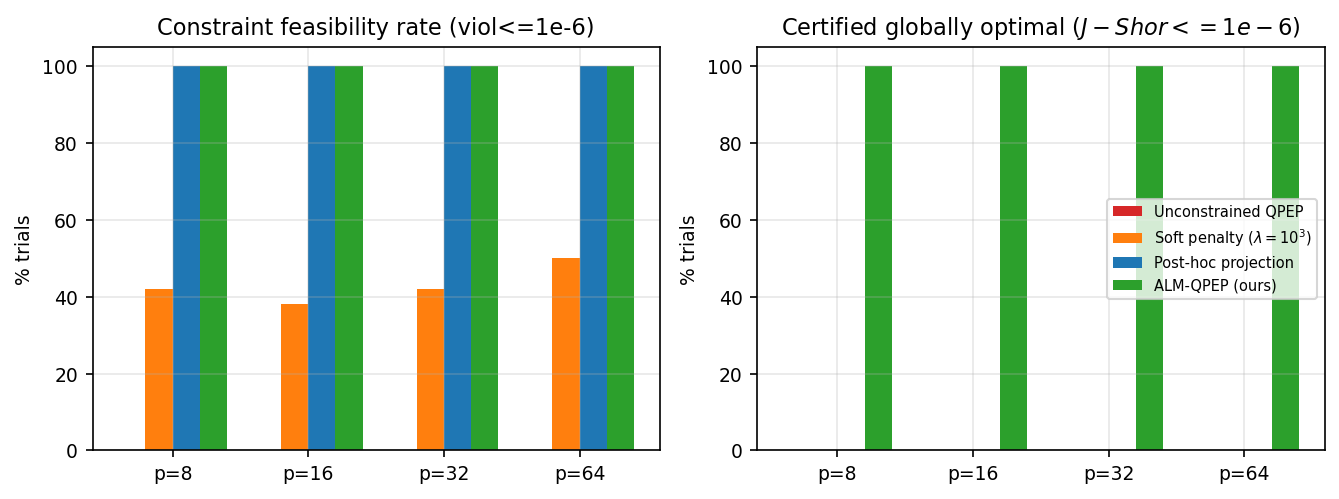
\includegraphics[width=\columnwidth]{fig_main_cert.png}
\caption{合成主扫描：约束可行率（左）与认证全局最优率（右）随 $p$ 的变化，每格 50 次试验。ALM-QPEP 在每个 $p$ 下 100\% 可行且 100\% 认证；投影可行但从未认证；软惩罚在 38--50\% 的试验中可行且从未认证。来源：\texttt{results/raw\_main.json}。}
\label{fig:app_cert}
\end{figure}

\subsection{噪声、偏置与惩罚的代价}\label{app:noise}
表~\ref{tab:app_noise} 固定 $p=16$，在四个格上变化逐点噪声 $\sigma$ 与竖直偏置。表~\ref{tab:app_pareto} 是在 $p=16$ 下对惩罚权重 $\lambda$ 的独立 50 次试验扫描。

\begin{table*}[t]
\centering
\caption{$p=16$ 下的方法 $\times$ 噪声/外参偏置（每格 50 次试验；中位 [IQR]）。}
\label{tab:app_noise}
\scriptsize
\setlength{\tabcolsep}{3pt}
\begin{tabular}{@{}llcccccc@{}}
\toprule
格（$\sigma$ / 偏置） & 方法 & 穿透 (mm) & 旋转 (deg) & 平移 (mm) & 可行 & 认证 \\
\midrule
0.000 / 0.000 & 无约束 QPEP & 0.00 [0.00, 0.00] & 0.00 [0.00, 0.00] & 7.07 [7.07, 7.07] & 100\% & 100\% \\
 & 软惩罚 & 0.00 [0.00, 0.00] & 0.00 [0.00, 0.00] & 7.07 [7.07, 7.07] & 100\% & 100\% \\
 & 事后投影 & 0.00 [0.00, 0.00] & 0.00 [0.00, 0.00] & 7.07 [7.07, 7.07] & 100\% & 100\% \\
 & ALM-QPEP & 0.00 [0.00, 0.00] & 0.00 [0.00, 0.00] & 7.07 [7.07, 7.07] & 100\% & 100\% \\
\midrule
0.005 / 0.040 & 无约束 QPEP & 47.52 [38.74, 51.36] & 2.52 [1.58, 3.25] & 45.87 [40.56, 51.75] & 0\% & 0\% \\
 & 软惩罚 & 0.01 [0.00, 0.03] & 5.10 [3.45, 7.36] & 9.46 [8.10, 11.27] & 24\% & 0\% \\
 & 事后投影 & 0.00 [0.00, 0.00] & 2.18 [1.75, 3.16] & 7.79 [7.12, 8.58] & 100\% & 0\% \\
 & ALM-QPEP & 0.00 [0.00, 0.00] & 2.52 [1.89, 3.33] & 8.46 [7.10, 9.65] & 100\% & 100\% \\
\midrule
0.010 / 0.080 & 无约束 QPEP & 103.02 [84.69, 110.83] & 5.30 [3.26, 6.70] & 97.90 [88.42, 107.73] & 0\% & 0\% \\
 & 软惩罚 & 0.00 [0.00, 0.03] & 6.62 [3.70, 9.95] & 13.00 [8.69, 16.87] & 38\% & 0\% \\
 & 事后投影 & 0.00 [0.00, 0.00] & 4.16 [2.90, 5.34] & 9.10 [7.34, 10.94] & 100\% & 0\% \\
 & ALM-QPEP & 0.00 [0.00, 0.00] & 4.17 [2.74, 5.10] & 10.63 [8.17, 12.69] & 100\% & 100\% \\
\midrule
0.020 / 0.120 & 无约束 QPEP & 198.10 [177.14, 232.79] & 11.50 [7.92, 18.63] & 185.77 [170.38, 215.92] & 0\% & 0\% \\
 & 软惩罚 & 0.00 [0.00, 0.04] & 11.13 [6.89, 14.36] & 17.01 [10.99, 21.60] & 38\% & 0\% \\
 & 事后投影 & 0.00 [0.00, 0.00] & 7.97 [5.45, 11.86] & 12.61 [8.90, 17.11] & 100\% & 0\% \\
 & ALM-QPEP & 0.00 [0.00, 0.00] & 5.83 [4.49, 7.55] & 13.39 [10.23, 17.43] & 100\% & 100\% \\
\bottomrule
\end{tabular}

\smallskip
\parbox{\textwidth}{\scriptsize 来源：\texttt{results/raw\_main.json}，\texttt{agg\_noise}，每格 50 次试验；软惩罚取 $\lambda=10^3$。}
\end{table*}

\begin{table}[t]
\centering
\caption{$p=16$ 下的软惩罚 Pareto（独立 50 次试验扫描；中位数）。}
\label{tab:app_pareto}
\footnotesize
\begin{tabular}{@{}lcccc@{}}
\toprule
$\lambda$ & 穿透 (mm) & 旋转 (deg) & 平移 (mm) & 可行 \\
\midrule
$10^0$ & 8.72 & 4.34 & 13.32 & 0\% \\
$10^1$ & 2.39 & 5.74 & 11.24 & 0\% \\
$10^2$ & 0.22 & 6.24 & 12.00 & 26\% \\
$10^3$ & 0.00 & 6.61 & 12.53 & 50\% \\
$10^4$ & 0.00 & 6.85 & 12.94 & 48\% \\
\bottomrule
\end{tabular}

\smallskip
\parbox{\columnwidth}{\scriptsize 来源：\texttt{results/raw\_main.json}，\texttt{pareto}（250 次试验 = 5 个权重 $\times$ 50 个种子）；数值与 \texttt{results/main\_table.md} 一致。}
\end{table}

三点观察。\textbf{(i) 无噪声格隔离了注入偏置。} 当 $\sigma=0$ 且竖直偏置为零时，四种方法完全一致：0.00~mm 穿透、$0.00^\circ$、7.07~mm 平移，均 100\% 可行且认证。7.07~mm 是固定的 5~mm 横向偏置（$\sqrt{5^2+5^2}=7.07$~mm），不是方法差异；没有噪声时约束不活跃。\textbf{(ii) 噪声与偏置把可行性与精度分开。} 在三个非零格上，无约束穿透从 47.52~$\to$~198.10~mm 增长且从不可行；ALM 在全部四格保持 0.00~mm、100\% 可行与认证；软惩罚在三个非零格中仅在 24--38\% 的试验中可行且从未认证；投影在那里 100\% 可行且从未认证。低噪声时三种受约束方法的位姿误差相当。在最高格上 ALM 的旋转误差最好（$5.83^\circ$，对无约束 $11.50^\circ$、软惩罚 $11.13^\circ$、投影 $7.97^\circ$），但投影的平移最好（12.61~mm 对 ALM 13.39~mm）；差异在离散范围之内。稳健效应是可容许性与认证，不是精度。\textbf{(iii) 更大的惩罚降低中位穿透，但从未达到可行性。} 表~\ref{tab:app_pareto}：中位穿透从 $\lambda=10^0$ 的 8.72~mm 单调降至 $\lambda=10^3$ 的 0.00~mm，代价是旋转误差从 $4.34^\circ$ 升至 $6.85^\circ$（平移基本持平，11.24--13.32~mm）。可行性从未超过 50\%，且非单调（$\lambda=10^3$ 时 50\%，$10^4$ 时 48\%）：惩罚逼近硬可行性但未达到。50 个种子中有一个对每个 $\lambda\ge10$ 都落入坏局部极小；$\lambda=10^4$ 时其旋转误差为 $132.9^\circ$、平移 202.6~mm，$\lambda=10^3$ 时平移误差 504.6~mm。这些离群值在中位数中不可见，也是惩罚路径无法被认证的原因。

\begin{figure}[t]
\centering
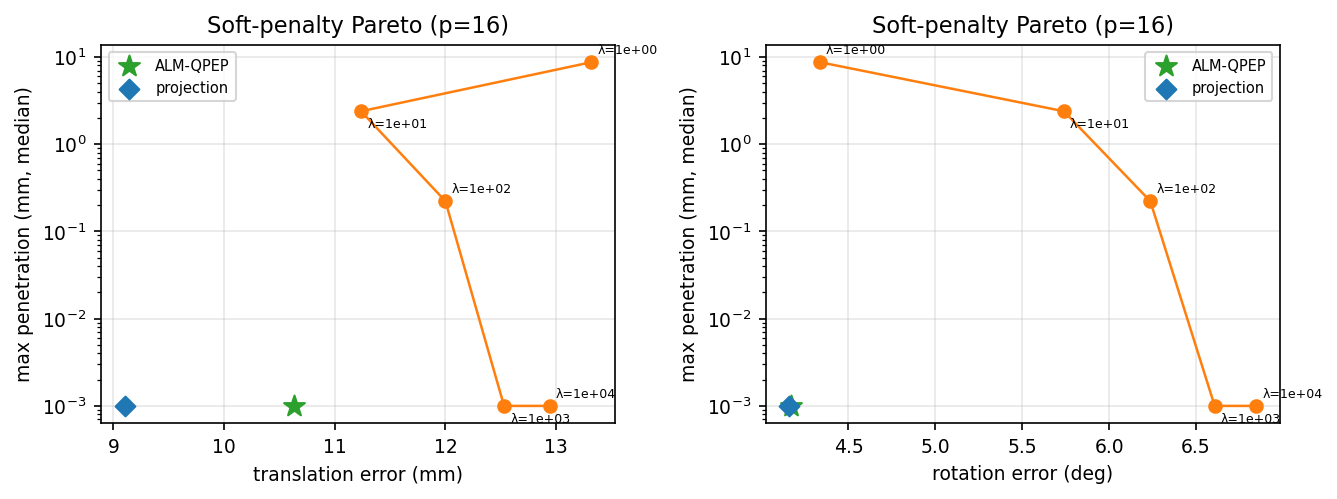
\includegraphics[width=\columnwidth]{fig_pareto.png}
\caption{$p=16$ 下的软惩罚 Pareto：$\lambda$ 在 $10^0$--$10^4$ 间变化时，中位最大穿透对平移误差（左）与对旋转误差（右）。ALM-QPEP（星）与投影（菱形）作为参考。来源：\texttt{results/raw\_main.json}，\texttt{pareto}。}
\label{fig:app_pareto}
\end{figure}

\begin{figure}[t]
\centering
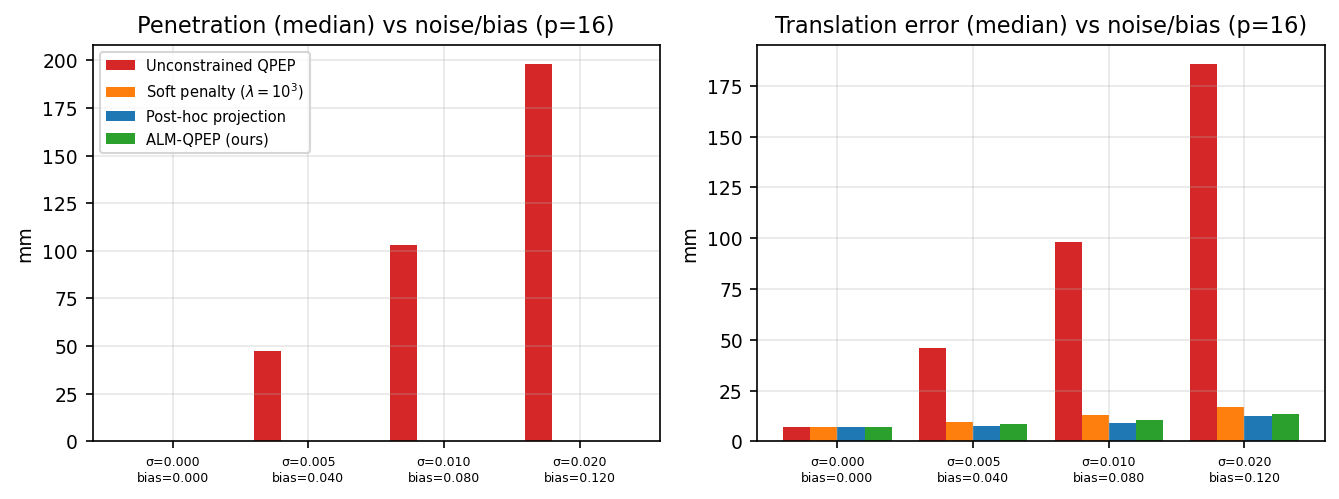
\includegraphics[width=\columnwidth]{fig_noise.png}
\caption{$p=16$ 下四种方法的中位穿透（左）与中位平移误差（右）随噪声/偏置格的变化。来源：\texttt{results/raw\_main.json}，\texttt{agg\_noise}。}
\label{fig:app_noise}
\end{figure}

\subsection{证书裕量、Schur 修复与 RLT 消融}\label{app:cert}
\begin{table*}[t]
\centering
\caption{全部 400 个合成实例（8 格 $\times$ 50）上的证书裕量。}
\label{tab:app_margins}
\scriptsize
\setlength{\tabcolsep}{3pt}
\begin{tabular}{@{}lcccccc@{}}
\toprule
格 & $n$ & $\max\lambda_2/\lambda_1$ & 中位 $\lambda_2/\lambda_1$ & $\mathrm{Shor}-J_{\rm ALM}$ 范围 & SDP 时间（均值，ms） \\
\midrule
主 $p=8$ & 50 & $1.42\times10^{-9}$ & $9.07\times10^{-11}$ & $[-4.56, 4.29]\times10^{-9}$ & 52.9 \\
主 $p=16$ & 50 & $1.03\times10^{-9}$ & $9.47\times10^{-11}$ & $[-3.28, 7.52]\times10^{-9}$ & 57.6 \\
主 $p=32$ & 50 & $8.43\times10^{-10}$ & $2.94\times10^{-11}$ & $[-5.66, 5.99]\times10^{-9}$ & 70.0 \\
主 $p=64$ & 50 & $1.51\times10^{-9}$ & $9.56\times10^{-11}$ & $[-3.93, 9.41]\times10^{-9}$ & 85.5 \\
噪声 $0.000/0.000$ & 50 & $5.55\times10^{-10}$ & $1.93\times10^{-11}$ & $[-8.78, 3.57]\times10^{-9}$ & 62.5 \\
噪声 $0.005/0.040$ & 50 & $8.56\times10^{-10}$ & $7.65\times10^{-11}$ & $[-6.31, 2.67]\times10^{-9}$ & 61.2 \\
噪声 $0.010/0.080$ & 50 & $1.03\times10^{-9}$ & $9.47\times10^{-11}$ & $[-3.28, 7.52]\times10^{-9}$ & 56.7 \\
噪声 $0.020/0.120$ & 50 & $1.08\times10^{-9}$ & $2.28\times10^{-11}$ & $[-4.25, 6.82]\times10^{-9}$ & 57.6 \\
\bottomrule
\end{tabular}

\smallskip
\parbox{\textwidth}{\scriptsize 来源：\texttt{results/cert\_margins.json}（由 \texttt{results/raw\_main.json} 汇总）。}
\end{table*}

合成松弛以很大裕量保持紧：全部 400 个实例中最大的 $\lambda_2/\lambda_1$ 为 $1.5\times10^{-9}$，比 $10^{-6}$ 阈值低约三个数量级，因此表~\ref{tab:app_main_rates} 与表~\ref{tab:app_noise} 无噪声格的 100\% 认证率不是勉强通过。$\mathrm{Shor}-J_{\rm ALM}$ 位于 $\pm10^{-8}$ 内且改变符号；这是 SCS 容差而非理论间隙，严格的可靠性主张需要定理~\ref{thm:cert} 的对偶可行修复。证书代价随 $p$ 从 8 到 64 由 52.9 增至 85.5~ms（均值；中位 51~$\to$~84），与固定的 $14\times14$ PSD 块加 $p$ 个线性约束一致。

\begin{table}[t]
\centering
\caption{定理 P2-Cert 的精确 Schur 界与保守 $P$-shift 对偶修复（6 个合成实例，$\sigma\in\{0.10,0.20\}$，$p=16$）。}
\label{tab:app_schur}
\scriptsize
\setlength{\tabcolsep}{3pt}
\begin{tabular}{@{}ccccc@{}}
\toprule
$\sigma$ & 种子 & $J$ & $J-\text{对偶修复}$ & $J-\text{Schur}$ \\
\midrule
0.10 & 0 & 9.0579e-01 & $2.00\times10^{-8}$ & $5.59\times10^{-12}$ \\
0.10 & 1 & 6.8500e-01 & $2.00\times10^{-8}$ & $-6.69\times10^{-13}$ \\
0.10 & 2 & 4.3643e-01 & $2.00\times10^{-8}$ & $5.31\times10^{-11}$ \\
0.20 & 0 & 3.2392e+00 & $2.04\times10^{-8}$ & $4.22\times10^{-10}$ \\
0.20 & 1 & 3.1128e+00 & $2.00\times10^{-8}$ & $3.81\times10^{-11}$ \\
0.20 & 2 & 3.0309e+00 & $2.01\times10^{-8}$ & $6.21\times10^{-11}$ \\
\bottomrule
\end{tabular}

\smallskip
\parbox{\columnwidth}{\scriptsize 来源：\texttt{results/p2b\_schur\_check.json}/\texttt{.md}（独立检查，\texttt{shor\_bound(..., schur=True)}；不修改 \texttt{certificate.py}）。六行均为 case~A。}
\end{table}

两个界都是可靠的；$13\times13$ 平移 Schur 补大约紧四个数量级。$P$-shift 修复因界定 $\|\mathbf t\|$ 而付出 $2c$ 损失，故其间隙固定在 $2\delta_{\rm round}\approx2\times10^{-8}$，而 Schur 界不需要 $\|\mathbf t\|$ 界，在六行中的五行留下 $5.6\times10^{-12}$--$4.2\times10^{-10}$。第六行记录 $J-d_{\rm sound}=-6.7\times10^{-13}$：这正是定理 P2-Cert 减去的浮点裕量 $\delta_{\rm round}\sim10^{-12}\|\mathbf S_{10}\|_F$ 的量级，即认证裕量水平上的舍入残差，而非结构性过冲——论文报告原始差，不把它舍入成“正”。结论：\texttt{rigorous\_schur} 是记录的界；$P$-shift \texttt{repair\_dual} 值仅作为保守回退保留（也是附录~\ref{app:baselines} 中 16/16 合成结果所引用的值，该结果早于 Schur 路径）。六行均为 case~A（$3\times3$ 平移块正定），故使用的是定理中较紧的分支。

\begin{table*}[t]
\centering
\caption{四个噪声水平下的零维 RLT 消融（每格 4 个种子）。}
\label{tab:app_rlt}
\scriptsize
\setlength{\tabcolsep}{2pt}
\begin{tabular}{@{}lcccccccc@{}}
\toprule
$\sigma$ / 偏置 & $n$ & 基础认证 & +RLT 认证 & 基础中位绝对间隙 & +RLT 中位绝对间隙 & 基础时间 (s) & RLT 时间 (s) \\
\midrule
0.02 / 0.10 & 4 & 4/4 & 4/4 & $1.6\times10^{-10}$ & $8.1\times10^{-11}$ & 0.05 & 0.15 \\
0.05 / 0.20 & 4 & 4/4 & 4/4 & $1.7\times10^{-9}$ & $9.4\times10^{-10}$ & 0.05 & 0.14 \\
0.10 / 0.30 & 4 & 1/4 & 2/4 & $4.2\times10^{-4}$ & $2.9\times10^{-4}$ & 1.59 & 0.85 \\
0.20 / 0.40 & 4 & 0/4 & 0/4 & $8.6\times10^{-3}$ & $7.8\times10^{-3}$ & 1.62 & 2.40 \\
\bottomrule
\end{tabular}

\smallskip
\parbox{\textwidth}{\scriptsize 来源：\texttt{experiments/theory/results/rlt.json}（16 个实例；全部 16 个可行）。}
\end{table*}

零维 RLT 割 $g_ig_j\ge0$（$p=16$ 时 136 行）只在基础间隙小到适度收紧即可越过阈值时有帮助，其余情形没有：
\begin{itemize}
\item 在 $\sigma=0.02$ 与 $0.05$ 时基础证书已是 4/4，RLT 不改变任何东西。
\item 在 $\sigma=0.10$ 时基础认证 1/4；RLT 认证 2/4。增益来自一个种子，其间隙从 $2.4\times10^{-4}$ 降至 $7.6\times10^{-12}$；已认证种子保持认证，其余两个仍以 $3.1\times10^{-3}$ 与 $5.8\times10^{-4}$ 的间隙未认证。
\item 在 $\sigma=0.20$ 时两种方法都认证 0/4。RLT 把逐种子间隙降低 10--17\%（中位 $8.6\times10^{-3}\to7.8\times10^{-3}$），仍比 $10^{-6}$ 容差高约四个数量级。
\item 在低噪声格上 RLT 证书约为基础 SDP 的 $3\times$（0.05~$\to$~0.15~s），在高噪声格上每实例 0.1--2.6~s，那里两个求解都不精确。
\end{itemize}
$\sigma=0.10$ 与 $0.20$ 的失败正是本稿不声称零维 RLT 闭合间隙的原因。可靠的高阶 bound-RLT 族在合成格上确实闭合了它（附录~\ref{app:baselines}）；其真实数据对应物是附录~\ref{app:real} 报告的严格重跑。

\textbf{适用哪种内层根计数。} 上述所有合成格使用 PnP 型基座，即定理~\ref{thm:spectrum} 的 Type~I：约简矩阵秩亏（$\sigma=0.01$ 时秩 9，$\sigma=0$ 时秩 8），但内层 KKT 系统仍具有 $N_{\mathbb C}=40$ 个复射影根与一般的 15-单项式 grevlex 阶梯，因为平移 $\mathbf M\mapsto\mathbf M+\alpha\mathbf I$ 只使 $f$ 改变 $\alpha(\mathbf q^\top\mathbf q)^2$，所有临界点保持不变。同伦算法每实例只找到 16--18 个\emph{实}根（\texttt{results/quartic\_validation.json}；早先一次运行引用 15--16），这是预期的 Type-I 图景，不是模板缺失的症状。紧致族则不同：各向同性 3D--3D（Horn）基座加 $k$ 个共享同一法向的活跃平面约束，在 $k=0/1/\ge2$ 时坍缩为 $N_{\mathbb C}=4/12/16$（Hopf 直纹线 $\mathcal L_{\mathbf n}$ 是必须饱和的多余分量），两个不同法向时为 $32$，各向异性/PnP 基座加任意平面时回到 $40$。在实现层面，只交付并端到端运行\textbf{一个}模板——用于一般/PnP 情形的 40 根未饱和模板。各向同性单平面情形（$k\ge2$；$k=1$ 为 12 根，$k=0$ 为 $4\times4$ Davenport）的 16 根\emph{饱和}模板仅\textbf{在用户证明中代数地}建立：$4/12/16$ 谱\textbf{在标准形下数值地}确认，而 $16\times16$ 饱和作用矩阵在本仓库中\textbf{未构建为已交付的数值模板}。拥有该族的模块用 162 路径同伦加多起点回退求解实例，而不是 16 根模板。因此我们\textbf{不}声称“两种规模的固定小模板”：我们的主张是 40 根模板在 Type-I 实例上实现并验证，$4/12/16$ 谱在标准形下数值验证，生产用 16 根数值模板部分存在/缺失。附录~\ref{app:baselines} 中的精确枚举计时仅在 Type-I 实例上测量。

\subsection{真实数据层结果}\label{app:real}
\begin{table*}[t]
\centering
\caption{真实数据层实验（$p=16$，真值投影对应；$n=90/72/84$）。}
\label{tab:app_real}
\scriptsize
\setlength{\tabcolsep}{3pt}
\resizebox{\textwidth}{!}{%
\begin{tabular}{@{}llccccccc@{}}
\toprule
数据集 & $n$ & 方法 & 穿透 (mm) & 旋转 (deg) & 平移 (mm) & 可行 & 单边（上界） & 双边（必要） \\
\midrule
LINEMOD & 90 & 无约束 QPEP & 11.26 & 2.08 & 35.63 & 13.3\% & 13.3\% & 8.9\% \\
 & & 软惩罚（$\lambda{=}10^3$） & 0.00 & 2.13 & 39.81 & 88.9\% & 26.7\% & 16.7\% \\
 & & 事后投影 & 0.00 & 2.05 & 30.80 & 100\% & 15.6\% & 10.0\% \\
 & & \textbf{ALM-QPEP（本文）} & \textbf{0.00} & \textbf{1.97} & \textbf{37.66} & \textbf{100\%} & \textbf{33.3\%} & \textbf{18.9\%} \\
\midrule
LM-O & 72 & 无约束 QPEP & 14.93 & 2.07 & 34.69 & 6.9\% & 6.9\% & 6.9\% \\
 & & 软惩罚（$\lambda{=}10^3$） & 0.00 & 1.90 & 39.91 & 91.7\% & 26.4\% & 9.7\% \\
 & & 事后投影 & 0.00 & 2.04 & 31.29 & 100\% & 8.3\% & 6.9\% \\
 & & \textbf{ALM-QPEP（本文）} & \textbf{0.00} & \textbf{1.99} & \textbf{38.14} & \textbf{100\%} & \textbf{30.6\%} & \textbf{12.5\%} \\
\midrule
YCB-Video & 84 & 无约束 QPEP & 14.09 & 1.08 & 17.33 & 6.0\% & 6.0\% & 3.6\% \\
 & & 软惩罚（$\lambda{=}10^3$） & 0.00 & 1.40 & 29.38 & 90.5\% & 21.4\% & 7.1\% \\
 & & 事后投影 & 0.00 & 1.08 & 8.93 & 100\% & 7.1\% & 4.8\% \\
 & & \textbf{ALM-QPEP（本文）} & \textbf{0.00} & \textbf{1.11} & \textbf{25.18} & \textbf{100\%} & \textbf{33.3\%} & \textbf{9.5\%} \\
\bottomrule
\end{tabular}}

\smallskip
\parbox{\textwidth}{\scriptsize 来源：\texttt{real/linemod/results/raw.json}、\texttt{real/bop/results/lmo/raw.json}、\texttt{real/bop/results/ycbv/raw.json}（$n=90/72/84$）；Wilson 置信区间见各 \texttt{main\_table.md}；软惩罚取 $\lambda=10^3$。单边标志为 $J-\mathrm{Shor}\le10^{-6}$，接受负间隙；双边标志为 $|J-\mathrm{Shor}|\le10^{-6}$。二者都不是严格证书：SCS 不是对偶可行的。严格替代见表~\ref{tab:rigorous}。}
\end{table*}

六点观察。\textbf{(i) 无约束求解在真实物体/桌面几何上不可行。} 它在 86.7\%（LM）、93.1\%（LM-O）与 94.0\%（YCB-Video）的行上违反可行性，中位穿透 11.26/14.93/14.09~mm。ALM 在三个数据集上 100\% 可行且穿透 0.00~mm；软惩罚在 88.9\%/91.7\%/90.5\% 的试验中可行。投影也 100\% 可行。\textbf{(ii) 约束买来的是可容许性，不是精度。} 四种方法都在 $1.1$--$2.1^\circ$ 旋转与 9--40~mm 平移内。ALM 并不比投影更精确（LM 平移 37.66 对 30.80~mm，LM-O 38.14 对 31.29~mm，YCB-Video 25.18 对 8.93~mm）。\textbf{(iii) 真实认证受上界限制且依赖数据集。} 单边 ALM 率为 33.3\% [24.5,43.6]（LM）、30.6\% [21.1,42.0]（LM-O）、33.3\% [24.2,43.9]（YCB-Video）；双边率为 18.9\%、12.5\%、9.5\%。零维 RLT 割\textbf{没有}给出可复现的真实增益：LM 33.3~$\to$~31.1（McNemar $p=0.85$），LM-O 30.6~$\to$~33.3（$p=0.86$），YCB 33.3~$\to$~23.8（$p=0.15$，更差）；在双边检验上 RLT 处处更差（18.9~$\to$~14.4，12.5~$\to$~4.2，9.5~$\to$~6.0）。因此我们把真实数据上的\emph{零维} RLT 报告为\textbf{负结果}。\textbf{(iv) 存储的真实数据证书标志是单边的。} 它检验 \texttt{feasible and J - Shor <= 1e-6}，不记录 $\lambda_2/\lambda_1$ 或 SDP 状态，并接受负间隙。在缩放运行中，18--26\% 的基础 ALM 行具有负间隙，双边率为 9.5--18.9\%。因此表~\ref{tab:app_real} 中的比率是\textbf{上界}；严格替代见表~\ref{tab:rigorous}。\textbf{(v) 严格认证与唯一正面的 RLT 结果。} 表~\ref{tab:rigorous} 用\emph{已证明}的下界替代两个标志：\texttt{rigorous\_schur}（13 维平移 Schur 补，记录的界），以及作为保守回退的 $P$-shift \texttt{repair\_dual} 值。计数在每个数据集上验证夹逼（单边 $\ge$ 严格 $\ge$ 双边）。\textbf{(vi) LM-O 纯平面行为何需要交叉方向割。} 见附录~\ref{app:lmo}。

五点解读。\emph{(a) 严格率远低于单边上界}——LM 24.4\% 对 33.3\%，LM-O 15.3\% 对 30.6\%，YCB-Video 13.1\% 对 33.3\%——并一致高于双边必要性检验（18.9/12.5/9.5）。夹逼顺序符合要求，上界与可靠率之间的差距（9--20 个百分点）正是单边标志所报告的数值假象大小。\emph{(b) 未认证行是真正的松弛，不是数值失败。} Schur 间隙在全部 738 个重放行上非负（3 个割族 $\times$ 246 个实例；0 个负间隙，最小 $4.0\times10^{-12}$--$1.7\times10^{-11}$，处于舍入下限），基础配置上的中位间隙为 $9.1\times10^{-6}$/$1.6\times10^{-5}$/$2.1\times10^{-5}$——是 $10^{-6}$ 容差的 9--21$\times$。紧性而非舍入，才是真实数据上的约束性限制。\emph{(c) 真实数据上 Schur 界与 $P$-shift 界相差 1--2 行}（22 对 23、11 对 11、11 对 10），不同于合成高噪声格上的四个数量级差距（表~\ref{tab:app_schur}）；逐行看，Schur 值在 82/90、68/72 与 78/84 个基础行上是两者中较紧的，且全部 738 个重放行都是 case~A（$\tilde{\mathbf H}_{tt}\succ0$，最大条件数 1668），因此使用的是定理 P2-Cert 的紧分支，没有行需要 $R_t$ 球。原因见上一点：当间隙 $\ge10^{-5}$ 时，$P$-shift 的 $2\delta_{\rm round}\approx2\times10^{-8}$ 代价无关紧要。我们仍把 Schur 值报告为记录的界、把 $P$-shift 值作为回退，因为只要间隙达到舍入下限，顺序就相反（Schur 更紧）。\emph{(d) 单边计数在不同 SDP 重解之间不可复现。} 在相同实例上（ALM $J$ 位级相同），重放在 \texttt{eps=1e-9}、50k 次迭代（存储运行为 20k）下重解 SDP，其值差异中位 $2.3\times10^{-8}$、最大 $3.7\times10^{-2}$；把\emph{同一} $J-\mathrm{Shor}\le10^{-6}$ 规则应用于重放值得到 25/90、19/72、17/84，而存储表报告 30/90、22/72、28/84。一个自身计数在不同求解间移动 5--11 行的检验不是证书，这就是论文把它降为仅上界的原因。\emph{(e) 可靠 bound-RLT 是正面结果，早先的负面结论来自不可靠的值。} 与基础配置相比，可靠的高阶 bound-RLT 族在 Schur 界上把严格认证从 22~$\to$~46（LM）、11~$\to$~30（LM-O）、11~$\to$~20（YCB-Video）提高——$+26.7/+26.4/+10.7$ 个百分点——McNemar $p=8.4\times10^{-6}$、$1.6\times10^{-4}$、$3.5\times10^{-2}$（配对标志；$0\to1$ 翻转 27/22/12，对 $1\to0$ 翻转 3/3/3）。在更保守的 $P$-shift 界上，相同计数为 23~$\to$~43、11~$\to$~24、10~$\to$~19（$+22.2/+18.1/+10.7$~pp；配对检验仅在 Schur 值上报告）。在同一可靠规则下零维族为零或负增益（Schur 22~$\to$~19、11~$\to$~6、11~$\to$~6；$p=0.45/0.063/0.063$）。在\emph{存储值}上，零维 RLT 看似在 LM-O 上有帮助（22~$\to$~24），只是因为它把 22/72 行的值推到 $J$ 以上；用可靠界后这一表面增益消失，而被不可靠标志判为失败的 bound-RLT 族，才是真正闭合间隙的那个。

\subsection{LM-O 深度与倾角增广}\label{app:lmo}
定理~\ref{thm:cert} 的结构性诊断指出：当每个活跃约束共享桌面法向时，RLT 乘积只约束 $\mathbf n^\top\mathbf t$，留下一个可容许的秩 2 伪混合；正深度与倾角锥行补上切割它的交叉方向块。表~\ref{tab:app_lmo} 在基础配置下 Schur 间隙最大的六个 LM-O 行上检验该预测（全部为帧 000002，物体 5/8/12，偏置 20/30~px；72 个基础行中有 61 个未认证）。

\begin{table*}[t]
\centering
\caption{LM-O 深度+倾角增广，前 $\to$ 后（6 个最差的基础未认证行）。}
\label{tab:app_lmo}
\scriptsize
\setlength{\tabcolsep}{3pt}
\resizebox{\textwidth}{!}{%
\begin{tabular}{@{}lccccc@{}}
\toprule
行（帧/图/物体/偏置） & 基础间隙 & bound-RLT 间隙（无增广） & 增广+基础间隙 & 增广+bound-RLT 间隙 & 增广后认证 \\
\midrule
000002/1/8/30 & $2.56\times10^{-4}$ & $1.45\times10^{-4}$ & $2.54\times10^{-4}$ & $9.0\times10^{-12}$ & 是 \\
000002/0/8/30 & $2.56\times10^{-4}$ & $2.00\times10^{-4}$ & $2.37\times10^{-4}$ & $5.2\times10^{-11}$ & 是 \\
000002/1/5/30 & $1.78\times10^{-4}$ & $3.54\times10^{-5}$ & $1.77\times10^{-4}$ & $1.0\times10^{-11}$ & 是 \\
000002/0/5/30 & $1.15\times10^{-4}$ & $1.0\times10^{-10}$ & $1.15\times10^{-4}$ & $9.9\times10^{-11}$ & 是 \\
000002/0/8/20 & $1.02\times10^{-4}$ & $6.17\times10^{-5}$ & $1.02\times10^{-4}$ & $1.9\times10^{-11}$ & 是 \\
000002/0/12/30 & $1.00\times10^{-4}$ & $9.37\times10^{-5}$ & $9.9\times10^{-5}$ & $6.0\times10^{-11}$ & 是 \\
\bottomrule
\end{tabular}}

\smallskip
\parbox{\textwidth}{\scriptsize 来源：\texttt{results/rigorous\_lmo\_depth\_tilt.json}（\texttt{run\_rigorous\_real.py depth-tilt --select worst --max-rows 6 --alpha 12 --n-depth 4}）；“无增广”列为 \texttt{real/bop/results/lmo/rigorous/rigorous\_rows.json} 中的行级 \texttt{brlt} 间隙。增广在 16 个平面行之外加入 4 个正深度行与 1 个直立锥行（$\alpha=12^\circ$，$\cos\alpha=0.978$）（$n_{\rm ineq}=16\to21$）。}
\end{table*}

预测以具体且可检验的形式成立。(a) 增广不改变答案：$|\Delta J|\le7.4\times10^{-15}$，且 ALM 的位姿已经满足新增行（最小深度 0.85--0.88~m $\gg z_{\min}=0.02$~m；直立度 0.998--0.999 $\ge\cos12^\circ$），因此证书针对的是具有相同最优解的问题，而非不同问题。(b) 仅增加行\emph{本身}无济于事：增广问题上的基础割仍在全部六行失败（间隙 $9.9\times10^{-5}$--$2.5\times10^{-4}$，基本不变）。(c) 在增广问题上使用 bound-RLT 后全部六行认证，间隙 $9\times10^{-12}$--$1.0\times10^{-10}$；不做增广时，单独 bound-RLT 只认证 6 行中的 1 行（该行为 $1.0\times10^{-10}$，其余为 $3.5\times10^{-5}$--$2.0\times10^{-4}$）。因此正是\emph{交叉方向 RLT 乘积} $g_{\rm plane}g_{\rm depth}$ 与 $g_{\rm plane}g_{\rm tilt}$ 承载增益，恰如定理所论证，深度/倾角行是促成者而非解药。诚实的范围：这是 61 个未认证 LM-O 行中的 6 行，按最差选取；这是机制检查，不是数据集级比率，数据集级比率仍为表~\ref{tab:rigorous} 中的值。

\subsection{基线、精确枚举与待完成项}\label{app:baselines}
\textbf{本轮测量。} 所有数字均为层级别，产生于共享登录节点；绝对计时随负载漂移，仅用于相对比较。

\begin{itemize}
\item \textbf{精确 QPEP 内层枚举，端到端穿过 ALM。} 在 $p\in\{8,16,64\}$ 的 8 次 ALM 试验上（$p=16$ 时种子 0--3，$p=8,64$ 时种子 0--1），精确 162 路径全次数枚举器与默认 6 起点多起点返回相同目标（$\max|\Delta J|=1.8\times10^{-12}$）、相同位姿（$\max\|\Delta\mathbf q\|=7.9\times10^{-10}$）、相同可行性（最大违反 $7.6\times10^{-11}$），且 7/8 次试验的外层迭代数相同（剩余 $p=64$ 试验提前一次迭代停止）。完备性是条件性的且经过测量：89/114 次枚举（78.1\%）找到一般 40 个有限射影根，25 次（21.9\%）丢失一条同伦路径并回退到 64 起点 BFGS；114 次探测枚举中每一次都有新的 64 起点 BFGS 达到同一全局极小。在 $\sigma=0.01$ 时 ALM 活跃集矩阵满秩（10/10，最小特征值 $8.2\times10^{-4}$），而无约束 $\mathbf M^{\rm red}_{\mathcal A}$ 秩为 9；无噪声矩阵秩为 8，有 16--18 个实根（\texttt{results/quartic\_validation.json}）。因此 25 次回退是同伦路径丢失，不是秩亏。精确内层每个位姿耗时 5.0--15.9~s，多起点为 0.12--0.28~s（37--64$\times$，中位 $47\times$）；混合调度（每三次外层迭代做一次精确枚举）在相同目标下将其降至 2.1--4.0~s。因此它买来的是固定活跃集下内层块的正确性/全局最优性检查，而不是有竞争力的内层求解器；默认仍是多起点。来源：\texttt{results/exact\_alm.json}、\texttt{.md}；仅内层的 24 实例表为 \texttt{results/quartic\_validation.json}。
\item \textbf{枚举代价更新（单独测量，未缩放）。} 上述 37--64$\times$ 比率是用优化前的枚举器测量的（一次 162 路径枚举平均 $\approx649$~ms）。同一代码的后续版本把形成 $\mathbf J^\top\mathbf M\mathbf J$ 的三操作数 \texttt{einsum} 替换为两次批量 BLAS 乘积（先 $\mathbf M\mathbf J$ 再 $\mathbf J^\top(\mathbf M\mathbf J)$，数学上等价），把一次枚举从 0.488~s 降至 0.168~s（2.92$\times$，356~$\to$~1077 路径/s），在 15 个案例上完全一致（相同根数、相同有限射影数，$\max|\Delta f|=3.3\times10^{-16}$），批量求值次数相同（中位 470）。由于此后\emph{未}重跑端到端 ALM 计时，我们\textbf{不}把 37--64$\times$ 范围除以 2.92：保留直接测得的 37--64$\times$ 作为保守数字，并把 2.92$\times$ 报告为孤立的内层循环加速。一个被否决的变体（提前剔除发散路径，\texttt{div\_tol} $10^3$--$10^2$）在 $10^3$ 时无收益、在 $10^2$ 时丢根，因此已回退。来源：\texttt{results/perf\_quartic.md}/\texttt{.json}。
\item \textbf{SCP 基线（dQP + 局部线性化）。} 在合成主格（$p=8/16/32$，各 50 次试验）上，SCP 100\% 可行，位姿误差与 ALM 在打印精度内一致（$p=16$：0.00~mm / $4.17^\circ$ / 10.63~mm），其输出在 98\% 的试验中通过同一 $14\times14$ 证书检验，而 ALM 为 100\%；它在此实现中更快（中位 130--142~ms 对 218--239~ms），约 90\% 墙钟时间花在 SOCP 上。在压力格（$\sigma=0.020$，偏置 0.120，20 次试验）上，SCP 认证 85\%，ALM 为 100\%。六次 SCP 失败都从手性镜像无约束解出发，且不能被额外两个扰动起点救回。因此我们声称的差异点是镜像初始化鲁棒性与 $p$ 无关的复杂度论证，而不是逐实例精度；SCP 是必须的强基线，并按此报告。来源：\texttt{results/scp\_baseline.md}（逐试验原始数据在 \texttt{results/scp\_baseline.json}）。
\item \textbf{可靠高阶 RLT（合成）。} 可靠 bound-RLT 族结合 \texttt{repair\_dual} 认证全部 16 个合成噪声实例（此前 9/16），最大严格间隙 $2.28\times10^{-8}$，证书时间中位 0.036~s $\to$ 0.180~s。增益集中在仅靠零维割失败处（$\sigma=0.10$：1/4~$\to$~4/4；$\sigma=0.20$：0/4~$\to$~4/4）。来源：\texttt{experiments/theory/results/round\_rlt.md}、\texttt{.json}。
\item \textbf{严格真实数据认证与 bound-RLT 结果。} 存储的单边标志在三个数据集上均被已证明的下界替代（表~\ref{tab:rigorous}）。基础配置：严格 Schur 22/90（24.4\%）、11/72（15.3\%）、11/84（13.1\%）——均低于单边上界（33.3/30.6/33.3\%），高于双边必要性检验（18.9/12.5/9.5\%）。Schur 界在全部 738 个重放行上非负（最小 $4.0\times10^{-12}$），因此失效模式是松弛：基础间隙中位为 $9.1\times10^{-6}$/$1.6\times10^{-5}$/$2.1\times10^{-5}$，是容差的 9--21$\times$。加入可靠 bound-RLT 族后严格率升至 46/90（51.1\%）、30/72（41.7\%）、20/84（23.8\%），即在 Schur 界上 $+26.7/+26.4/+10.7$~pp（在 $P$-shift 计数上 $+22.2/+18.1/+10.7$~pp），配对 McNemar $p=8.4\times10^{-6}$、$1.6\times10^{-4}$、$3.5\times10^{-2}$，SDP 代价 0.9--1.5$\times$，Schur 修复 0.20--0.36~ms。零维 RLT 族在同一可靠规则下仍为零或负增益（Schur 22~$\to$~19、11~$\to$~6、11~$\to$~6；$p=0.45/0.063/0.063$）。这推翻了早先“RLT 在真实数据上为负”的解读：\textbf{零维 RLT 是负结果；可靠 bound-RLT 是真实增益}。来源：\texttt{results/rigorous\_lm.json}、\texttt{results/rigorous\_lmo.json}、\texttt{results/rigorous\_ycbv.json}，以及 \texttt{results/rigorous\_real.\{json,md\}}。
\end{itemize}

\textbf{仍待完成。} 以下内容被刻意排除，第~\ref{sec:intro}--\ref{sec:method} 节中的任何主张都不依赖它们：\emph{学习型与其余凸层基线}（无约束及带 $p$ 个松弛变量的 SDPRLayers、Theseus；dQP 族基线即上述 SCP 组合）；\emph{端到端训练}（附录~\ref{app:protocol} 的 T1-network、T2 与 T3 协议；ADD(-S)、真实帧上的穿透、KITTI/TUM/UTIAS）；\emph{反向传播与延迟拆分}（只计时前向求解；FB 反向传播、装配/内层/证书拆分，以及 Gauss--Newton 对精确 Hessian、FB $\varepsilon$、证书开关与内层求解器消融均未测量）；以及\emph{真实数据规模扩展}（真实表使用 $n=90/72/84$；Wilson 区间见附录~\ref{app:real}，RLT 差值在这些规模下不显著，故按负结果报告）。生产层（\texttt{torch.autograd.Function} 加参考 NumPy 实现）不属于本稿工件；实验在 \texttt{experiments/code/} 下运行研究实现。所有结果文件、聚合脚本与绘图脚本位于 \texttt{experiments/results/}；健全性检查脚本与输出位于 \texttt{verify/}。


\end{document}
